\documentclass[11pt]{article}
\usepackage{fullpage}
\usepackage{empheq}
\usepackage{color}
\usepackage {listings}
\usepackage{amsmath}
\usepackage{hyperref}
\usepackage{longtable}
\usepackage{array}
%\usepackage[scaled]{beramono}
\usepackage[T1]{fontenc}
\usepackage{tabularx}
\usepackage{amssymb}
\usepackage{enumitem}
\usepackage{booktabs}
\usepackage{multirow} 
\usepackage{tipa}

%\setmonofont{Consolas} %to be used with XeLaTeX or LuaLaTeX
\definecolor{bluekeywords}{rgb}{0,0,1}
\definecolor{blue(munsell)}{rgb}{0.0, 0.5, 0.69}
\definecolor{greencomments}{rgb}{0,0.5,0}
\definecolor{redstrings}{rgb}{0.64,0.08,0.08}
\definecolor{xmlcomments}{rgb}{0.5,0.5,0.5}
\definecolor{types}{rgb}{0.17,0.57,0.68}
\setlength\parindent{0pt}

\lstset{language=[Sharp]C,
captionpos=b,
%numbers=left, %Nummerierung
%numberstyle=\tiny, % kleine Zeilennummern
frame=lines, % Oberhalb und unterhalb des Listings ist eine Linie
showspaces=false,
showtabs=false,
breaklines=true,
showstringspaces=false,
breakatwhitespace=true,
escapeinside={(*@}{@*)},
commentstyle=\color{greencomments},
morekeywords={partial, var, get, set,string,false,true},
keywordstyle=\color{bluekeywords},
stringstyle=\color{redstrings},
basicstyle=\ttfamily\small,
}
\lstset%
{%
    emph=[1]%
    {%
        Process,
        Cplex,
        Program,
        IntParam,
        NumVarType,
        INumVar,
        SystemInformation,
        Param,
        Stopwatch,
        Instance,
        ProcessStartInfo,
        Point,
        ILinearNumExpr,
        List,
        PathGenetic,
        Random,
        ILinearNumExpr,
        TSPLazyConsCallback,
        StreamWriter,
        IRange,
        itemList,
        DoubleParam,
        Convert,
        StringSplitOptions
    },
    emphstyle=[1]{\color{blue(munsell)}},
}


\begin{document}

ABSTRACT

\vspace{2\baselineskip}

Il presente progetto riguarda la progettazione di un software in grado di risolvere istanze del problema del Commesso Viaggiatore applicando differenti algoritmi risolutori. L'obiettivo di questo testo \`e quello di descrivere le tecniche utilizzate e di confrontare i risultati ottenuti in termini di efficienza e bont\`a della soluzione prodotta. Verr\`a fornita una descrizione degli strumenti e l'ambiente di sviluppo utilizzati e sar\`a analizzato il codice di programmazione realizzato; non mancheranno paragrafi dedicati ad approfondire concetti teorici senza i quali la comprensione del codice potrebbe risultare meno chiara. 

\vspace{2\baselineskip}
INTRODUZIONE 

\vspace{2\baselineskip}

Questa capitolo introduttivo \`e dedicato alla storia, alle applicazioni e alle correnti sfide riguardanti uno dei pi\`u importanti problemi che la disciplina di Ricerca Operativa si trova ad affrontare, ossia il problema del commesso viaggiatore(Travelling Salesman Problem-TSP). 
Il nome deriva dalla sua pi\`u tipica rappresentazione: data una rete di citt\`a, connesse tramite delle strade, si vuole trovare il percorso di minore distanza che un commesso viaggiatore deve seguire per visitare tutte le citt\`a una ed una sola volta e ritornare alla citt\`a di partenza. Per quanto detto, risulta naturale modellare il TSP come un grafo pesato i cui nodi modellizzano le citt\`a relative al problema in questione mentre i possibili collegamenti tra le localit\`a sono modellati con gli archi del grafo i cui pesi possono rappresentare,per esempio, la distanza esistente fra la coppia di nodi collegati dall' arco. Chiaramente \`e possibile assegnare i pesi in modo arbitrario secondo le nostre esigenze, ad esempio si potrebbe anche tenere conto dei tempi di percorrenza o di eventuali pedaggi presenti nei singoli percorsi. Come \`e facile immaginare, il TSP pu\`o essere quindi utilizzato per una infinit\`a  di problemi pratici ma anche teorici.\\
Il problema del commesso viaggiatore riveste un ruolo notevole nell' ambito di problemi di logistica distributiva, detti anche problemi di routing. Questi riguardano l'organizzazione di sistemi di distribuzione di beni e servizi. Esempi di problemi di questo genere sono la movimentazione di pezzi o semilavorati tra reparti di produzione, la raccolta e distribuzione di materiali, la distribuzione di merci da centri di produzione a centri di distribuzione.
Sebbene le applicazioni nel contesto dei trasporti siano le pi\`u naturali per il TSP, la semplicit\`a del modello ha portato a molte applicazioni interessanti in altre aree. Un esempio pu\`o essere la programmazione di una macchina per eseguire fori in un circuito. In questo caso i fori da forare sono le citt\`a  e il costo del viaggio \`e il tempo necessario per spostare la testa del trapano da un foro all'altro. 
Il problema del commesso viaggiatore risulta essere NP-hard: questo significa che, al momento, non \`e noto in letteratura un algoritmo che lo risolva in tempo polinomiale. Poich\`e esiste sempre una istanza per cui il tempo di risoluzione cresce esponenzialmente non \`e sempre possibile utilizzare algoritmi esatti per risolvere il TPS. Risulta quindi necessario fornire algoritmi euristici, in grado di risolvere in modo efficace istanze con un numero elevato di nodi in tempi ragionevoli.


Problemi matematici riconducibili al TSP furono trattati nell' Ottocento dal matematico irlandese Sir William Rowan Hamilton e dal matematico Britannico Thomas Penyngton.  Nel 1857, a Dublino, Rowan Hamilton descrisse un gioco, detto Icosian game, a una riunione della British Association for the Advancement of Science. Il gioco consisteva nel trovare un percorso che toccasse tutti i vertici di un icosaedro, passando lungo gli spigoli, ma senza mai percorrere due volte lo stesso spigolo. L'icosaedro ha 12 vertici, 30 spigoli e 20 facce identiche a forma di triangolo equilatero.
Il gioco, venduto alla ditta J. Jacques and Sons per 25 sterline, fu brevettato a Londra nel 1859, ma vendette pochissimo. Questo problema \`e un TSP nel quale gli archi che collegano vertici adiacenti, e quindi corrispondono a spigoli dell'icosaedro, sono consentiti e gli altri no (si pu\`o pensare che richiedano moltissimo tempo e quindi vadano sicuramente scartati), per tale ragione si tratta di un caso molto particolare di TSP. La forma generale del TSP fu invece studiata solo negli anni Venti e Trenta del ventesimo secolo dal matematico ed economista Karl Menger. Tuttavia, per molto tempo non si ebbe altra idea che quella di generare e valutare tutte le soluzioni, il che mantenne il problema praticamente insolubile. Il numero totale dei differenti percorsi possibili attraverso le $n$ citt\`a \`e facile da calcolare: data una citt\`a di partenza, ci sono a disposizione $(n - 1)$ scelte per la seconda citt\`a, $(n - 2)$ per la terza e cos\` via. Il totale delle possibili scelte tra le quali cercare il percorso migliore in termini di costo \`e dunque $(n - 1)!$, ma dato che il problema ha simmetria, questo numero va diviso a met\`a . Insomma, date n citt\`a, ci sono $\frac{(n-1)!}{2}$ percorsi che le collegano.

Solo nel 1954, George Dantzig, Ray Fulkerson e Selmer Johnson proposero un metodo pi\`u raffinato per risolvere il TSP  su un campione di $n = 49$ citt\`a: queste rappresentavano le capitali degli Stati Uniti e il costo del percorso era calcolato in base alle distanze stradali. 

Nel 1962, Procter and Gamble bandì un concorso per 33 citt\`a, nel 1977 fu bandito un concorso che collegasse le 120 principali citt\`a della Germania Federale e la vittoria and\`o a Martin Gr\"otschel oggi Presidente del Konrad-Zuse-Zentrum f\"ur Informarionstechnik Berlin(ZIB) e docente presso la Technische Universit\"at Berlin(TUB).

Nel 1987  Padberg e Rinaldi riuscirono a completare il giro degli Stati Uniti attraverso 532 citt\`a. Nello stesso periodo Groetschel e Holland trovarono il TSP ottimale per il giro del mondo che passava per 666 mete importanti. 
Nel 2001, Applegate, Bixby, Chvátal, and Cook trovarono la soluzione esatta a un problema di 15.112 citt\`a tedesche, usando il metodo cutting plane, originariamente proposto nel 1954 da George Dantzig, Delbert Ray Fulkerson e Selmer Johnson. Il calcolo fu eseguito da una rete di 110 processori della Rice University e della Princeton University. Il tempo di elaborazione totale fu equivalente a 22,6 anni su un singolo processore Alpha a 500 MHz.
Sempre Applegate, Bixby, Chv\a`tal, Cook, e Helsgaun trovarono nel Maggio del 2004 il percorso ottimale di 24,978 citt\`a della Svezia. 
Nel marzo 2005, il TSP riguardante la visita di tutti i 33.810 punti in una scheda di circuito fu risolto usando CONCORDE: fu trovato un percorso di 66.048.945 unit\`a, e provato che non poteva esisterne uno migliore. L'esecuzione richiese approssimativamente 15,7 anni CPU. 
Ai giorni nostri il risolutore Concorde per il problema del commesso viaggiatore \`e utilizzato per ottenere soluzioni ottime su tutte le 110 istanze della libreria TSPLIB; l' istanza con pi\`u nodi in assoluto ha 85,900 citt\`a. 

\vspace{2\baselineskip}

MODELLO MATEMATICO
\vspace{2\baselineskip}

Nella sua formalizzazione pi\`u generale, il problema del Commesso Viaggiatore consiste nell'individuare un circuito hamiltoniano di costo minimo per un dato grafo orientato $G=(V,A)$, dove $V = $\{$ {v_1,\dots,v_n} $\}$ $ \`e un insieme di $n$ nodi e $A = $\{$ {(i,j): i, j \in V} $\}$ $ \`e un insieme di $m$ archi\footnote{Chiaramente sia $n$ che $m$ sono interi positivi}. 

Senza perdita di generalit\`a, si suppone che il grafo $G$ sia completo e che il costo associato all'arco $[i,j]$, che indicheremo con $c_{ij}$, sia non negativo. Si osserva che aver imposto $c_{ij} \ge 0$ non \`e limitativo poich\'e \`e sempre possibile sommare a tutti i costi una costante sufficientemente elevata che li renda positivi senza alterarne l'ordinamento delle soluzioni. 
A differenza di quanto detto in precedenza, per tutto il proseguimento della tesi supporremmo il grafo $G$ non orientato: tale scelta deriva dal fatto che $c_{ij}$ nel nostro lavoro rappresenta sempre la distanza (tipicamente euclidea) fra i vertici i e j si ha che:
$$c_{ij} = c_{ji}$$

ossia il costo associato ad un arco non dipende dalla direzione dell'arco stesso. Quando il grafo \`e non orientato la famiglia di coppie non ordinate di elementi di V, ossia l'insieme degli archi, viene indicato con $E$.


Definito il problema forniamo ora una sua possibile formulazione in termini di PLI. Introducendo le seguenti variabili decisionali:

\[
x_{e}=
\begin{cases}
1 & \text{se il lato $e \in E$ viene scelto nel circuito ottimo} \\
0 & \text{altrimenti}
\end{cases}
\]

si ottiene il problema:

\begin{eqnarray}
& \text{min}\displaystyle\underbrace{\sum_{e \in E} c_e x_e}_{\text{costo circuito}} \\[1.5ex]
&\displaystyle\underbrace{\sum_{e \in \delta(V)} x_e = 2}_{\text{due lati incidenti in }v}\text{,  }\forall v \in V \\[1.5ex]
&0\leq x_e \leq 1 \text{ intera , }\forall e \in E
\end{eqnarray}

L' insieme di vincoli definiti dalla (2) vengono chiamati vincoli di grado e impongono che in ogni vertice incidano esattamente due lati. In questa forma il modello \`e  compatto dato che il numero di vincoli \`e polinomiale rispetto alla dimensione dell'istanza ma non \`e completo poich\'e \`e sprovvisto dei vincoli di subtour che impediscono soluzioni il cui grafo risulta non connesso.

\begin{center}
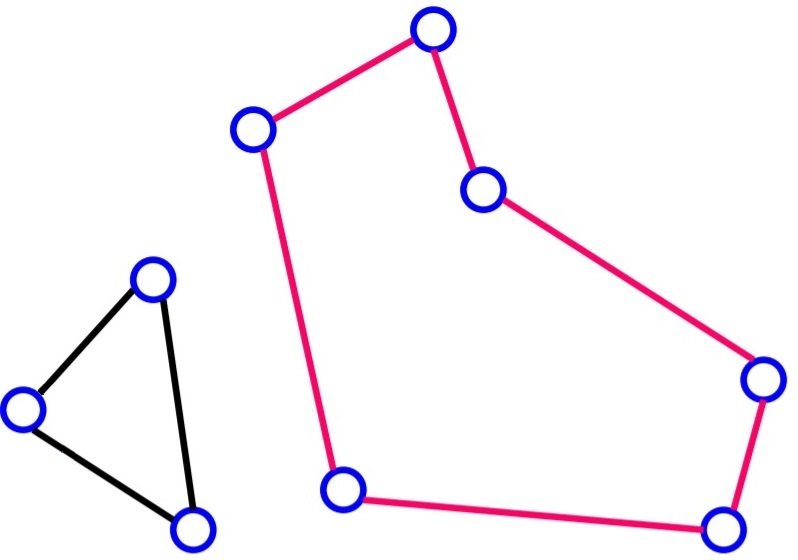
\includegraphics[scale=0.5]{subtour}  

Figura 1: Soluzione con due subtour
\end{center}

\vspace{2\baselineskip}

Una possibile formulazione per l'eliminazione dei subtour, detta appunto \textbf{subtour elimination}, risulta essere:

\begin{eqnarray}
&\displaystyle{\sum_{e \in E(S)}x_e \geq 1} \text{ , } \forall S \subsetneq V \text{ : } 1 \in S \text{ , } |S| \geq 2
\end{eqnarray}


Il vincolo (4) indica che se si considera un sottoinsieme $S \subsetneq V$, che includa il vertice numerato con il simbolo 1, allora il taglio di G indotto da S:

\begin{center}
$\delta(S) = $\{$ {[i,j]\in E : i \in S, j \notin S} $\} $ $
\end{center}

deve contenere almeno un lato appartenente ad $E$: poich\'e tutti i subtour violano tale vincolo la soluzione ottima non potr\`a contenerne al suo interno.  
Essendo il numero di questi vincoli pari ai sottoinsiemi $S$ distinti, il numero di tali vincoli risulta esponenziale rispetto alla dimensione dell'istanza. In particolare il valore di $S$, dato un numero $n$ di nodi, \`e $2^n$: questo perch\`e associando un bit ad ogni vertice (il cui valore definisce se appartiene o meno al sottoinsieme) un qualsiasi sottoinsieme risulta identificato da una sequenza di $n$ bit è quindi possibile definirne $2^n$ distinti. In realtà avendo noi imposto che il vertice 1 appartenga sempre ad ogni $S$ e che $S \subsetneq V$, si ha che il numero di vincoli di subtour risulti pari a  $2^{n-1} - 1$.

Una seconda formulazione equivalente per esprimere i vincoli di subtour \`e la seguente:

\begin{eqnarray}
&\displaystyle{\sum_{e \in E(S)}x_e \leq |S| - 1} \text{ , } \forall S \subsetneq V \text{ , } |S| \geq 2
\end{eqnarray}

La gestione di un numero esponenziale di vincoli implica in genere tempi di risoluzione troppo elevati. Nella pratica però non è necessario utilizzare tutti i vincoli di subtour elimination, è sufficiente considerarne un numero molto più ridotto. Non potendo conoscere in anticipo quali siano quelli essenziali sarà nostro compito progettare un opportuno separatore: ossia una funzione che fornita in ingresso una soluzione x* ottima per il modello corrente generi tutti i vincoli violati.


\vspace{2\baselineskip}
FILE DI INPUT
\vspace{2\baselineskip}


Le istanze del problema del Commesso Viaggiatore fornite in input al programma sono state selezionata da un libreria presente al seguente indirizzo web: 

\begin{center}
\href{http://elib.zib.de/pub/mp-testdata/tsp/tsplib/tsp/index.html}{http://elib.zib.de/pub/mp-testdata/tsp/tsplib/tsp/index.html}
\end{center}

Ogni istanza è memorizzata in un file di testo in un formato ben preciso, \`e stato quindi possibile progettare un opportuno parser che automaticamente riesca a estrapolare le informazioni contenute e popolare le strutture dati da noi create\footnote{Nessun altro tipo di input è supportato}. 

\vspace{2\baselineskip}



\vspace{2\baselineskip}
STRUTTURA DEL PROGETTO
\vspace{2\baselineskip}


I file che compongono il programma realizzato sono stati organizzati nel modo seguente; all' interno della cartella radice, da noi chiamata TSPCsharp, si sono create le seguenti sottocartelle:

\begin{itemize}
\item \textbf{Src} contenente il progetto di Visual Studio;
\item \textbf{Data} include le istanze del problema del commesso viaggiatore appartenenti alla TSPlib;
\item \textbf{Concorde} contenente i file sorgenti in linguaggio C del programma Concorde\footnote{Concorde è un software freeware sviluppato da \textbf{William Cook} per la risoluzione di problemi TSP} la cui trattazione \`e rimandata al Capitolo X.
\end{itemize}

Il software sviluppato \`e composto da dieci classi, riportiamo di seguito il nominativo di ognuna di esse:

\begin{itemize}
\item Instances
\item ItemList
\item PathGenetic
\item PathStandard
\item Point
\item Program
\item Tabu
\item TSP
\item TSPLazyConsCallback
\item Utility
\end{itemize}

Per le classi Point, Instances, Program, TSP e Utility verr\`a fornita una descrizione in questo capitolo, le rimanenti classi verranno presentate nei capitoli successivi poich\'e una loro trattazione risulterebbe in questo momento prematura. 


\vspace{2\baselineskip}
CLASSE POINT
\vspace{2\baselineskip}

La classe Point \`e stata realizzate al fine di memorizzare le coordinate in due dimensioni di un singolo nodo $n$, a tal fine sono presenti due variabili private, accessibili attraverso i propri metodi get e set, di tipo \textbf{double} chiamate rispettivamente \textbf{x} e \textbf{y}. Il costruttore della classe non fa altro che ricevere in input i valori da assegnare a queste ultime. La classe presenta inoltre un ulteriore metodo pubblico e statico chiamato \textbf{Distance} che permette il calcolo della distanza tra due nodi:

\begin{lstlisting}
    public static double Distance(Point p1, Point p2, string pointType)
\end{lstlisting}

\begin{itemize}
\item \textbf{p1}: Rappresenta il primo nodo;
\item \text{p2}: Rappresenta il secondo nodo;
\item \textbf{pointType}: Rappresenta il modo con cui il costo relativo al lato che congiunge p1 con p2 viene calcolato; i valori che questo parametro pu\`o assumere sono i seguenti:
	\begin{itemize}
	\item EUC\char`_2D
	\item ATT
	\item MAN\char`_2D
	\item GEO
	\item MAX\char`_2D	
	\item CEIL\char`_2D
	\end{itemize}
\end{itemize}

A titolo di esempio riportiamo il codice eseguito nel caso in cui pointType risulti uguale a EUC\char`_2D dove il costo del lato deve risultare pari alla distanza euclidea dei due nodi. 

\begin{lstlisting}

 double xD = p1.X - p2.X;
 double yD = p1.Y - p2.Y;
 
 if (pointType == "EUC_2D")
 {
     return (int)(Math.Sqrt(xD * xD + yD * yD) + 0.5);
 }
 else if ...
            
\end{lstlisting}

Per quanto riguarda gli altri metodi di calcolo della distanza rimandiamo il lettore alla visione del codice.

\vspace{2\baselineskip}
CLASSE INSTANCE
\vspace{2\baselineskip}

La classe Instance \`e stata creata per memorizzare tutti i dati caratterizzanti l'istanza del problema del Commesso Viaggiatore. La tabella sottostante fornisce un elenco di variabili ed array definite all'interno della classe assieme ad una loro breve descrizione. 


\begin{center}

    \begin{longtable}{ | p{4cm} | p{4cm} | p{7cm} |}
    \hline
    \begin{center} \textbf{Tipo di dato} \end{center} & \begin{center}  \textbf{Nome} \end{center}& 
    \begin{center} \textbf{Descrizione} \end{center}\\ \hline
    \begin{center} int \end{center} & \begin{center} nNodes \end{center}& \vfill Rappresenta il numero di nodi dell' istanza del problema del Commesso Viaggiatore.\vfill \\ \hline
    \begin{center} Point[ ] \end{center} & \begin{center} coord \end{center}& \vfill Vettore di Point contenente le coordinate di tutti i vertici del grafo.\vfill\\ \hline
    \begin{center} string \end{center} & \begin{center} edgeType \end{center}&\vfill Definisce la modalit\`a con cui calcolare la distanza fra due nodi.\vfill \\ \hline
    \begin{center} double \end{center} & \begin{center} timeLimit \end{center}& \vfill Definisce la quantit\`a massima di tempo che il programma dispone per il calcolo della soluzione.\vfill \\ \hline
    \begin{center} double \end{center} & \begin{center} inputFile \end{center}&\vfill Rappresenta il nome del file di input contenente l'istanza del problema del Commesso Viaggiatore. \vfill\\ \hline
    \begin{center} double \end{center} & \begin{center} tStart \end{center}& \vfill Rappresenta i secondi trascorsi dall'attivazione del cronometro al reale inizio delle operazioni di calcolo per la risoluzione del problema \vfill \\ \hline
    \begin{center} double \end{center} & \begin{center} xBest \end{center}& \vfill Rappresenta il costo della soluzione ottima restituira da cplex.\vfill \\ \hline
    \begin{center} double \end{center} & \begin{center} tBest \end{center}& \vfill Contiene la qantit\`a di tempo impiegata per il calcolo della soluzione ottima. \vfill \\ \hline
    \begin{center} double \end{center} & \begin{center} bestSol \end{center}& \vfill Rappresenta la soluzione ottima ritornata da Cplex.\vfill \\ \hline
     \begin{center} double \end{center} & \begin{center} bestLb \end{center}& \vfill Rappresenta il miglior lower bound attualmente calcolato.\vfill \\ \hline
    \begin{center} double \end{center} & \begin{center} bestLb \end{center}& \vfill Rappresenta il miglior lower bound attualmente calcolato.\vfill \\ \hline
     \begin{center} double \end{center} & \begin{center} bestLb \end{center}& \vfill Rappresenta il miglior lower bound attualmente calcolato.\vfill \\ \hline
    \end{longtable}
\end{center}

\textit{xMin e yMin ... mi servivano per gnuplot ma dato che ho messo l'autoscale credo non servano più. per xBest ok}

L' unico metodo appartenente a questa classe, esclusi i vari getter e setter, è \textbf{Print}, la cui firma risulta essere:

\begin{lstlisting}
                  static public void Print(Instance inst)
\end{lstlisting}

dove:

\begin{itemize}
\item \textbf{inst}: oggetto della classe Instance contente tutti dati che descrivono l'istanza del problema del Commesso Viaggiatore fornita in ingresso dall' tente;
\end{itemize}

Tale metodo stampa a video le coordinate di tutti i nodi memorizzati dentro \textbf{inst}. Viene di seguito riportato il codice:

\begin{lstlisting}
for (int i = 0; i < inst.NNodes; i++)
    Console.WriteLine("Point #" + (i + 1) + "= (" + inst.Coord[i].X + "," + inst.Coord[i].Y + ")");
\end{lstlisting}

\vspace{2\baselineskip}

CLASSE PROGRAM

\vspace{2\baselineskip}

La classe Program contiene il metodo Main che, come noto, rappresenta il punto di inizio del programma: attraverso le funzionalità di Visual Studio esso riceve in input l'array \textbf{argv} di stringhe contenente i parametri di input forniti dall'utente come il nome del file contenente l'input ed il time limit per la sua risoluzione. Appartengono a questa classe anche i metodi \textbf{ParseInst} e \textbf{Populate}: rispettivamente forniscono il parser per \textbf{argv} ed il parser del file di ingresso indicato con conseguente inizializzazione delle coordinate dei nodi. Firma e implementazione di tali metodi \`e rimandata al successivo capitolo.\\
All'interno del metodo \textbf{Main} vengono eseguite in ordine le seguenti attività:
\begin{itemize}
	\item Creata una istanza della classe \textbf{Instance} ed invocati i due metodi precedentemente nominati.
	\item Creato un oggetto della classe \textbf{Stopwatch}. Questa classe è fornita direttamente da Visual Studio appartenente al Namespace \textbf{System.Diagnostics} è fornisce le funzionalità di un cronometro compatibile al multithreading.
	\item Invocato il metodo \textbf{TSPOpt} della classe \textbf{TSP} passandogli come parametri i due oggetti di tipo Instance e Stopwatch.
	\item In caso di risultato positivo (una soluzione del problema è stata trovata) viene mostrato a video il risultato ottenuto ed il tempo di calcolo trascorso.
	\item Viene effettuata una pulizia dei file creatisi durante l'esecuzione del problema.
\end{itemize}

In tutto il nostro progetto si è cercato di utilizzare il minor numero possibile di variabili globali, in particolare solo all'interno di questa classe ne sono state definite due di seguito descritte:

\begin{center}
	
	\begin{tabular}{ | p{1.5cm} | p{4cm} | p{2cm} | p{6.5cm} |}
		\hline
		\begin{center} \textbf{Tipo di dato} \end{center} & \begin{center}  \textbf{Nome} \end{center}& \begin{center} \textbf{Valore} \end{center} & \begin{center} \textbf{Descrizione} \end{center}\\ \hline
		\begin{center} int \end{center} & \begin{center} VERBOSE \end{center}& \begin{center} 5 \end{center} & Regola quanto output il programma mostra a video: si \`e scelto di condizionare l' esecuzione di molte righe di codice che producevano una stampa a video in base al valore assunto da questa variabile. Si \`e deciso di ristringere il suo valore da 1 a 9, quando assume il valore 9 viene riportato a video il maggior numero possibile di stampe. \\ \hline
		\begin{center} int \end{center} & \begin{center} TICKS\char`_PER\char`_SECOND \end{center} &  \begin{center}1000  \end{center}& Cplex utilizza i così detti ticks come unità di misura per il tempo di calcolo, questa costante indica quanti ne trascorrono in un secondo.\\ \hline
		
	\end{tabular}
\end{center}

\vspace{2\baselineskip}
CLASSE TSP
\vspace{2\baselineskip}

La classe \textbf{TSP} è stata pensata come il cuore del programma in quanto lo scheletro di tutti i metodi di risoluzione implementatisi trova al suo interno. Contiene un unico metodo pubblico che rappresenta quindi l'unico entry point per utilizzare questa classe: \textbf{TSPOpt}.

\begin{lstlisting}
static public bool TSPOpt(Instance instance, Stopwatch clock)
\end{lstlisting}

Come già specificato nella descrizione della classe Program, TSPOpt è invocato dal metodo Main e pertanto maggiori dettagli riguardanti i suoi parametri di ingresso possono essere trovati nella sezione precedente.\\
TSPOpt si preoccupa di istanziare i vari elementi utilizzati da tutti i metodi di risoluzione\footnote{Fatta eccezione per l'UserCutCallBack che è gestita esternamente da una DLL}, fornire all'utente un'interfaccia grafica che gli permetta di scegliere quale di questi ultimi voglia utilizzare e di conseguenza invoca il metodo privato della classe associato alla scelta effettuata.\\
Entrando nello specifico per quanto riguarda gli elementi inizializzati troviamo un oggetto della classe \textbf{Cplex} che come già accennato in precedenza ci permetterà di stabilire una connessione con il programma Cplex ed utilizzarlo per la risoluzione del modello matematico, ed un oggetto \textbf{Process} che sostanzialmente viene da noi utilizzato per inizializzare e comunicare con il programma \textbf{GNUPlot}\footnote{Per maggiori dettagli si veda la sezione dedicata a GNUPlot}.

\vspace{2\baselineskip}
CLASSE UTILITY
\vspace{2\baselineskip}

La classe Utility può essere considerata come una libreria: contiene al suo interno solamente metodi \textbf{statici} che si è deciso di raggruppare al suo interno per rendere il codice il più compatto e leggibile possibile.

\vspace{2\baselineskip}
INTERPRETAZIONE FILE DI INPUT
\vspace{2\baselineskip}

Lo sviluppo del programma \`e iniziato realizzando una opportuna funzione per interpretare correttamente i parametri di ingresso forniti dall'utente. Oltre al nome del file di testo contenente i dati relativi  all'istanza del problema che si vuole risolvere, all'utente \`e richiesto di fornite un time limit(espresso in secondi) e di scegliere con quale algoritmo risolvere l'istanza da esso fornita. Si \`e deciso di ricevere da riga di comando il nome del file e il time limit; per quanto riguarda la scelta dell'algoritmo risolutore ed eventuali parametri da esso richiesti si \`e preferito realizzare una semplice interfaccia grafica per favorire l'utente. 
Visual Studio, all'interno delle proprietà del progetto, permette di definire una stringa come parametro di ingresso per il programma. Questa viene automaticamente separata in sottostringhe utilizzando come separatore il carattere di spazio e fornito in ingresso al metodo Main. Allo stato attutale è gestita solamente la possibilità di fornire in ingresso il nome del file contenente i dati ed il timelimit per la ricerca della soluzione. Per ottenere una migliore organizzazione e chiarezza per il nostro lavoro è stato deciso di utilizzare questa regola per la costruzione della stringa di ingresso: ogni parametro inseritovi deve essere preceduto da una parola chiave che lo identifica il cui primo carattere deve essere '-'. Questa tecnica si rileverà utile anche in futuro nel caso si decidesse di ampliare la lista di parametri di ingresso.\\
La funzione che interpreta correttamente gli argomenti forniti in input dalla riga di comando \`e stata chiamata ParseInst ed ha la seguente intestazione:

\begin{lstlisting}
	  static void ParseInst(Instance inst, string[] input) 
\end{lstlisting}


\begin{itemize}
\item \textbf{inst}: rappresenta il riferimento all'istanza della classe Instance dichiarata nel metodo Main, i valori letti vengono memorizzati al suo interno.
\item \textbf{input}: rappresenta un vettore contenente i parametri di input forniti da riga di comando dall'utente.
\end{itemize}


Il metodo \`e composto da un semplice ciclo for che scandisce il vettore \textbf{input} cercando una parola chiave, se trovata la stringa successiva viene memorizzata correttamente dentro \textbf{inst}: 

\begin{lstlisting}

for (int i = 0; i < input.Length; i++)
{
   if (input[i] == "-file")
   {
     //Expecting that the next value is the file name
       inst.InputFile = input[++i];
       continue;
    }
    if (input[i] == "-timelimit")
    {
      //Expecting that the next value is the time limit in seconds
       inst.TimeLimit = Convert.ToDouble(input[++i]);
       continue;
    }
}   			
\end{lstlisting}

Nel caso in cui l' utente non fornisca il nome del file di input oppure il time limit viene lanciata una eccezione:

\begin{lstlisting}

if (inst.InputFile == null || inst.TimeLimit == 0)
     throw new Exception("File input name and/or timelimit are missing");

\end{lstlisting}


\vspace{2\baselineskip}
METODO POPULATE
\vspace{2\baselineskip}

Il metodo Populate \`e utilizzato per la lettura dei dati contenuti all'interno del file di input e soprattutto alla loro memorizzazione all'interno di un oggetto di tipo \textbf{Instance} in modo tale che una volta conclusosi il metodo questo contenga tutte le informazioni necessarie per la creazione del modello matematico.\\
I file di input presenta una struttura pressoché identica tra loro e cioè una divisione in sezioni identificate da parole chiave. Fatta eccezione per la sezione che descrive le coordinate dei nodi, tutte le altre si sviluppano in una sola riga la cui struttura \'e del tipo:

\begin{center}
<parolaChiave> : < valore> 
\end{center}

Di seguito sono riportati i valori che possono essere assunti dalle parole chiavi e il significato del contenuto della relativa sezione: 

\begin{itemize}
	\item NAME:<string> 
	\begin{itemize}
	\item nome con cui l' istanza \`e nota in letteratura.
	\end{itemize}
	\item TYPE:<string>
	
	\begin{itemize}	 
	\item indica il tipo dell' istanza. Nel nostro ambito sar\`a sempre TSP.    
    \end{itemize}	
	 
	\item \textbf{COMMENT:<string>} 
	\begin{itemize}	
	\item include informazioni aggiuntive, solitamente contiene il nome deli gli autori che hanno proposto l'  				istanza.
	\end{itemize}	
	
		
	\item \textbf{DIMENSION:<integer>} 
	\begin{itemize}
	\item indica il numero di nodi.
	\end{itemize}	
	
	\item \textbf{EDGE WEIGHT TYPE:<string>}
	\begin{itemize} 
	\item Definisce il modo con cui il costo del lato deve essere calcolato, i possibili valori  che pu\'o assumere    		     il contenuto di questa sezione sono stati gi\`a presentati a pagina 7 durante la descrizione del metodo Distance.
	\end{itemize}	
	
	\item \textbf{NODE COORD SECTION}: 
	\begin{itemize}	
	
	\item Il contenuto di questa sezione si sviluppa in pi\`u righe; in ogni riga troviamo nell' ordine:
	\begin{itemize}
	\item Un numero progressivo intero positivo che comincia da 1 e che identifica il nodo. Osserviamo che anche se in input il primo nodo \`e numerato a partire da 1, nel vettore Point di inst le coordinate saranno memorizzate a partire dall'indice 0\footnote{Tale scelta \'e per mantenere una conformit\'a con la metrica adottata dal linguaggio C\# per l'enumerazione degli elementi dei vettori, nel caso in cui le coordinate vengano visualizzate a video il loro indice viene comunque incrementato di uno}.
	\item Un numero reale positivo che definisce la coordinata x del nodo.
	\item Un numero reale positivo che identifica la coordinata y del nodo.
	\end{itemize}		
	\end{itemize}	
\end{itemize}

Il file di testo termina sempre con la stringa \textbf{EOF} che indica la fine del file di testo.

Per poter leggere il contenuto di un file \`e necessario inizializzare una nuova istanza della classe StreamReader passando come parametro al costruttore il percorso ove tale file \`e  collocato.


\begin{lstlisting}

StreamReader sr = new StreamReader("..\\..\\..\\..\\Data\\" + inst.InputFile)

\end{lstlisting}


Il metodo ReadLine() della classe StreamReader ritorna, come stringa, il contenuto di una intera riga del file la quale viene memorizzata all'interno di una variabile di tipo string chiamata \textbf{line}. Poich\'e si vuole leggere tutto il contenuto del file, \`e necessario invocare ReadLine() ciclicamente sull' oggetto \textbf{sr} finch\`e line risulta diversa da null oppure viene incontrata la parola chiave \textbf{EOF}.

\begin{lstlisting}

while ((line = sr.ReadLine()) != null)
{
	...
	
	//This line signals the end of the file
	if (line.StartsWith("EOF"))
	{
	Instance.Print(inst);
	Console.WriteLine(line);
	//Correct end of the file
	break;
	}
	
	...
}
\end{lstlisting}


Poich\'e ogni riga inizia con una nota parola chiave, per prelevare il contenuto di una sezione e memorizzarlo in un opportuno campo di inst, \`e sufficiente confrontare la prima stringa di ogni riga con una delle noti parole chiavi. Per far ci\`o si \`e  usato il metodo StartWith della classe String, la cui firma \`e:

\begin{lstlisting}

                    public bool StartWith(string value)

\end{lstlisting}

Questo metodo, applicato alla variabile line, determina se la prima stringa di line corrisponde alla stringa value specificata all'atto dell' invocazione del metodo. Nel caso in cui il confronto dia esito positivo, per prelevare il contenuto della sezione \`e necessario applicare i metodi IndexOf e Remove sempre alla variabile line; l'intestazione di tali metodi \`e riportata di seguito:


\begin{lstlisting}

               public int IndexOf(string value,int startIndex)

\end{lstlisting}

dove:

\begin{itemize}
	\item \textbf{value}: stringa da cercare.
	\item \textbf{startIndex}: posizione iniziale della ricerca.
\end{itemize}

\begin{lstlisting}

                public string Remove(int startIndex, int count)

\end{lstlisting}


dove:

\begin{itemize}
	\item \textbf{startIndex}: posizione da cui iniziare l'eliminazione dei caratteri.
	\item \textbf{count}: numero di caratteri da eliminare.
\end{itemize}

Per quanto detto, risulta immediata la comprensione del codice necessario per prelevare il contenuto della sezione e memorizzarlo dentro un oggetto di tipo \textbf{Instance} chiamando il metodo setter adeguato:

\begin{lstlisting}

                inst.SetterName = (line.Remove(0, line.IndexOf(:) + 2));

\end{lstlisting}

Il codice riportato deve chiaramente effettuare un cast per i tipi diversi da string, i metodi necessari sono già disponibili all'interno della classe \textbf{Convert} di C\#.

Una volta che ci troviamo all'interno della sezione \textbf{NODE COORD SECTION} la lettura delle coordinate viene eseguita eseguendo ciclicamente il seguente codice:

\begin{lstlisting}

string[] elements = line.Split(new[]{ ' ' } , StringSplitOptions.RemoveEmptyEntries);

int i = Convert.ToInt32(elements[0]);

inst.Coord[i - 1] = new Point(Convert.ToDouble(elements[1].Replace(".", ",")), Convert.ToDouble(elements[2].Replace(".",",")));
\end{lstlisting}

Il metodo Split della classe String ritorna un array contenente in ogni elemento una sottostringa della stringa a cui tale metodo \`e applicato. Le sottostringhe vengono estratte dalla stringa in base ai caratteri delimitatori specificati all'atto dell'invocazione del metodo, quest'ultimo ha diversi overload: quello di nostro interesse \`e riportato di seguito.

\begin{lstlisting}

     public string[] Split(char[] separator, StringSplitOptions options)

\end{lstlisting}

dove:

\begin{itemize}
\item \textbf{separator}: array i cui elementi definiscono i separatori della stringa. Nel nostro caso è un array con un solo elemento contenente il carattere \textipa{"}   \textipa{"}.
\item \textbf{options}: A questo parametro possono essere passate solo i seguenti due valori dell' enumerazione StringSplitOptions:

\begin{itemize}

\item \textbf{StringSplitOptions.RemoveEmptyEntries}: indica che gli elementi dell'array ritornato non possono essere stringhe vuote. Questo è l'opzione da noi selezionata.
\item \textbf{StringSplitOptions.None}: indica che gli elementi dell'array ritornato possono essere stringhe vuote.

\end{itemize}

\end{itemize}

Ogni coordinata letta viene tradotta in un oggetto di tipo \textbf{Point} il quale è a sua volta memorizzato all'interno del vettore \textbf{Coord} dell'oggetto di tipo \textbf{Instance} nella posizione indice letta.

Come nota conclusiva specifichiamo che C\# utilizza come separatore tra parte intere e parte decimale di un numero il carattere \textipa{"},\textipa{"} e non il carattere \textipa{"}.\textipa{"} utilizzato per nei file di input. E' quindi necessaria una modifica delle stringhe lette attraverso il metodo non statico della classe string:

\begin{lstlisting}

     public string Replace(string oldValue, string newValue)
)

\end{lstlisting}
dove:
\begin{itemize}
	\item \textbf{oldValue}: stringa sa sostituire;
	\item \textbf{newValue}: stringa con cui sostituire tutte le occorrenze di oldValue.
\end{itemize}

\vspace{2\baselineskip}
COSTRUZIONE DEL MODELLO
\vspace{2\baselineskip}

In questo paragrafo vedremo come \`e possibile creare da programma un modello matematico attraverso l'uso di alcune routine appartenenti alla libreria di Cplex. Esula dallo scopo di questa tesi fornire al lettore una descrizione del funzionamento di Cplex da iterativo.


\vspace{2\baselineskip}
COSTRUZIONE MODELLO IN C
\vspace{2\baselineskip}

Per istanziare un nuovo modello di programmazione lineare \`e necessario inizializzare un \textbf{environment} di Cplex utilizzando la funzione \textbf{CPXopenCPLEX} la quale ritorna un puntatore all'environment creato, la firma di tale funzione \`e:


\begin{lstlisting}

                CPXENVptr CPXopenCPLEX(int* status_p)

\end{lstlisting}

dove:

\begin{itemize}
\item \textbf{status\char`_p}: puntatore ad una variabile di tipo intero usato per ritornare un eventuale codice di errore.
\end{itemize}


Ad un enviroment è possibile associare uno o pi\`u modelli attraverso il comando \textbf{CPXcreateprob}, la cui intestazione \`e:

\begin{lstlisting}

    CPXLPptr CPXcreateprob(CPXCENVptr env, int * status_p, const char * probname_str

\end{lstlisting}


dove:

\begin{itemize}
	\item \textbf{env}: puntatore all'environment sul quale si \`e deciso di creare il modello;
	\item \textbf{status\char`_p}: puntatore ad una variabile di tipo intero usato per ritornare un eventuale codice di errore;
	\item \textbf{probname\char`_str}: rappresenta un array di caratteri che definisce il nome del modello creato.
\end{itemize}

Tale funzione ritorna un puntatore al modello creato: questo risulta vuoto poich\`e privo di funzione obbiettivo, variabili e vincoli.\\

Procediamo quindi al loro inserimento partendo definendo contemporaneamente le variabili e il loro coefficiente nella funzione obiettivo; è possibile procedere in più modi, quello da noi scelto è di utilizzare la funzione \textbf{CPXnewcols} la cui firma \`e:


\begin{lstlisting}

int CPXnewcols (CPXENVptr env,CPXLPptr lp,int ccnt,double *obj, double *lb, double *ub, char *ctype, char **colname);

\end{lstlisting}

dove:

\begin{itemize}
\item \textbf{env} : puntatore all'enviroment di Cplex nel quale vuole essere inserito il modello.
\item \textbf{lp} : puntatore al problema di programmazione lineare.
\item \textbf{ccnt} : intero che indica il numero delle nuove variabili che vengono aggiunte al problema.
\item \textbf{obj} : array contenente per ogni variabile il relativo coefficiente 
\item \textbf{lb} : array di lunghezza ccnt contenente il lower bound di ogni variabile aggiunta.
\item \textbf{ub} : array contenente l'upper bound di ogni variabile aggiunta.
\item \textbf{ctype} : array di lunghezza ccnt contenente il tipo di ogni variabile. I valori che un elemento di questo array pu\`o assumere sono:
\begin{itemize}
	\item \textbf{\textipa{"}C\textipa{"}}: variabile continua
	\item \textbf{\textipa{"}B\textipa{"}}: variabile binaria
	\item \textbf{\textipa{"}I\textipa{"}}: variabile intera
\end{itemize}
\item \textbf{colname} : array di lunghezza ccnt contenente puntatori ad array di char, a sua volta ognuno di essi deve contenere il nome della variabile aggiunta al modello.
\end{itemize}

Per motivi di semplicità non andremo ad inserire tutte le variabili contemporaneamente ma una ad una.\\

E' giunto quindi il momento di parlare di quali variabili vogliamo aggiungere al nostro modello tenendo presente che il medesimo discorso sarà applicato anche per la parte in C\#. Sappiamo che per ogni coppia di nodi (i,j)\footnote{Ricordiamo che i deve essere diverso da j in quanto per i problemi da noi considerati i cappi non sono ammessi} esiste un unico lato che li collega e che quest'ultimo è privo di direzione. Si presenta quindi la necessità di definire una convenzione per l'assegnazione del nome ai vari lati. La scelta adottata è la seguente: considerando due generici nodi \textbf{i} e \textbf{j} allora il loro lato sarà chiamato \textbf{x(i,j)} se $i<j$ oppure \textbf{x(j,i)} se $j<i$\footnote{Notiamo che per quanto espresso nella nota precedente non ha senso considerare il caso $i=j$}.\\
Questa convenzione offre anche un importante spunto per decidere con quale ordine memorizzare i vari parametri delle variabili (nome, coefficiente, lower bound ecc..): date due coppie distinti di nodi (i,j) e (v,w)\footnote{dove assumiamo $i<j \& v<W$} la posizione di memoria in cui viene memorizzata l'informazione riguardante la prima coppia è \textbf{inferiore} rispetto alla seconda se e solo se $(i<v) || (i==v \& j<w)$. In altre parole saranno memorizzate in ordine le informazioni per i nodi (1,2), (1,3), ..., (2,3), (2,4), ..., (n-1,n).\\
Una ulteriore considerazione necessaria \'e la seguente: come mostrato poco fa il metodo \textbf{CPXnewcols} si aspetta il passaggio di diversi array mentre noi vorremmo utilizzare semplici variabili. La soluzione \'e molto semplice e consiste nell'anteporre il carattere \& prima di ogni variabile in questo modo stiamo in realtà passando un puntatore alla sua locazione di memoria.\\

Le operazioni descritte sono state realizzate tramite il seguente codice:

\begin{lstlisting}

double zero = 0.0; // one = 1.0; 	
char binary = 'B';

char **cname = (char **)calloc(1, sizeof(char *));		// (char **) required by cplex...
cname[0] = (char *)calloc(100, sizeof(char));

// add binary var.s y(i,j)      

for (int i = 0; i < inst->nNodes; i++)
{
	for (int j = i + 1; j < inst->nNodes; j++)//Mi interessano solo le coppie con i<j
	{
		sprintf(cname[0], "x(%d,%d)", i + 1, j + 1);
		double obj = dist(inst->coord[i], inst->coord[j], inst->edgeType);
		double ub = 1.0;
		if (CPXnewcols(env, lp, 1, &obj, &zero, &ub, &binary, cname)) printError(" ... errato CPXnewcols su x");//Aggiugo una variabile al modello
		if (CPXgetnumcols(env, lp) - 1 != xPos(i, j, inst)) printError(" ... errata posizione per x");//Serve solo per controllare se la funzione xPos è corretta
	}
}

\end{lstlisting}

La funzione chiamata xPos  riceve in ingresso un lato (i,j) del grafo e restituisce l'indice della variabile Cplex associata a quest'ultimo. Dato che risulta possibile effettuare errori nella realizzazione di questa funzione, in questo punto del codice \`e  utile effettuare un controllo se il valore ritornato da xPos coincide con quello aspettato,in caso contrario viene sollevata una eccezione. Firma e dettagli implementativi di xPos saranno forniti nel paragrafo successivo in quanto è definita anche in C\#.\\

Una volta definite le variabili \`e necessario creare i vincoli: per far ci\`o si \`e utilizzata la funzione \textbf{CPXnewrows}, la cui firma \`e:

\begin{lstlisting}
int CPXnewrows(CPXCENVptr env, CPXLPptr lp, int rcnt, const double * rhs, const char * sense, const double * rngval, char ** rowname)
\end{lstlisting}

dove:

\begin{itemize}
\item \textbf{env}: puntatore all'enviroment di Cplex nel quale vuole essere inserito il modello.
\item \textbf{lp}: puntatore al problema di programmazione lineare.
\item \textbf{rcnt}: intero che definisce il numero di nuovi vincoli aggiunti al modello.
\item \textbf{rhs}: array di lunghezza rcnt contenente il termine noto di ogni vincolo.
\item \textbf{sense}: array di lunghezza rcnt i cui elementi possono assumere i seguenti valori:

\begin{itemize}
\item \textbf{\textipa{"}L\textipa{"}}: indica che il vincolo \`e una disuguaglianza il cui segno \`e  $\leq$
\item \textbf{\textipa{"}E\textipa{"}}: indica che il vincolo \`e una uguaglianza
\item \textbf{\textipa{"}G\textipa{"}}: indica che il vincolo \`e una disuguaglianza il cui segno \`e $\geq$
\item \textbf{\textipa{"}R\textipa{"}} : indica che il vincolo \`e limitato 
\end{itemize}

\item \textbf{rngval}: variabile di tipo double contenente il valore 1.0;
\item \textbf{rowname}: variabile di tipo char che assume il valore costante \textipa{"}B\textipa{"};
\end{itemize}

Anche in questo caso anzich\`e aggiungere tutti i vincoli in una singola iterazione, risulta pi\`u semplice aggiungere un vincolo per volta invocando il metodo tante volte quante sono i vincoli da aggiungere.

\vspace{2\baselineskip}
COSTRUZIONE E RISOLUZIONE DEL MODELLO MATEMATICO IN C\#
\vspace{2\baselineskip}

Per poter creare un modello matematico in Cplex, utilizzando come linguaggio di programmazione C\# \`e necessario creare inizialmente una istanza della classe \textbf{Cplex}:

\begin{lstlisting}
                           Cplex cplex = new Cplex();
\end{lstlisting}

Per creare il modello si associano, tramite opportune funzioni che descriveremo in questo paragrafo, all'istanza creata la funzione obbiettivo,le variabili e i vincoli del modello. 

In C\# le variabili del modello sono oggetti il cui tipo deve implementare l'interfaccia \textbf{INumVar}. Non è necessario creare da noi una nuova classe infatti ci viene fornito il metodo \textbf{NumVar} della classe \textbf{Cplex}:

\begin{lstlisting}
public virtual INumVar NumVar(double lb, double ub, NumVarType type, string name)
\end{lstlisting}

dove:

\begin{itemize}
\item \textbf{lb}: Rappresenta il lower bound della variabile creata;
\item \textbf{ub}: Rappresenta l' upper bound della variabile creata;
\item \textbf{type}: Questo campo determina il tipo della variabile, pu\`o assumere i seguenti valori:
\begin{itemize}
\item \textbf{NumVarType.Int}: Nel caso di variabile intera;
\item \textbf{NumVarType.Int}: Nel caso di variabile binaria;
\item \textbf{NumVarType.Float}: Nel caso di variabile continua;
\end{itemize}
\item \textbf{name}: Nome identificativo della variabile.
\end{itemize}

Che come si può notare nella firma ha come tipo di ritorno un tipo di oggetto che implementa l'interfaccia da noi desiderata. Vedremo nel seguito della trattazione quanto utili risultano essere le funzionalità offerta de quest'ultima.\\
Introduciamo ora una seconda interfaccia \textbf{ILinearNumExpr} che come si può intuire viene implementata da oggetti che vogliono definire una espressione lineare. Anche in questo caso ci viene incontro la classe \textbf{Cplex} attraverso il metodo \textbf{LinearNumExpr}:
\begin{lstlisting}
                ILinearNumExpr expr = cplex.LinearNumExpr();
\end{lstlisting}

La variabile \textbf{expr} rappresenta quindi una espressione lineare che deve essere definita come:

$$\displaystyle{\sum_{i = 1}^n a_i x_i} $$

dove \textbf{$x_i$} sono variabili di tipo \textbf{INumVar} mentre \textbf{$a_i$} \'e un coefficiente di tipo \textbf{double}. Per aggiungere all'oggetto \textbf{expr} una variabile del modello \`e necessario utilizzare il metodo \textbf{AddTerm} la cui intestazione \`e:

\begin{lstlisting}
                   void AddTerm(INumVar var,double coef)
\end{lstlisting}

dove:

\begin{itemize}
\item \textbf{var}: variabile da aggiungere all'espressione;
\item  \textbf{coeff}: coefficiente della variabile aggiunta all'espressione.
\end{itemize}

L'implementazione da noi fornita per quanto riguarda la funzione obiettivo \'e la seguente:

\begin{lstlisting}
//Populating objective function

for (int i = 0; i < instance.NNodes; i++)
{
  //Only links (i,j) with i < j are correct
  
  for (int j = i + 1; j < instance.NNodes; j++)
  {
      //zPos returns the correct position where to store the variable corresponding to the actual link (i,j)
           
     int position = zPos(i, j, instance.NNodes);
           
     z[position] = cplex.NumVar(0, 1, NumVarType.Int, "x(" + (i + 1) + "," + (j + 1) + ")");
         
     expr.AddTerm(z[position], Point.Distance(instance.Coord[i], instance.Coord[j], instance.EdgeType));      
   }
}

\end{lstlisting}

Espressioni lineari definite in questo modo possono essere utilizzate sia per definire la funzione obiettivo del modello ma anche per i suoi vincoli.\\
Nel primo caso risulta sufficiente invocare i metodi non statici \textbf{AddMinimize} oppure \textbf{AddMaximize} della classe \textbf{Cplex} che rispettivamente definiscono una funzione obiettivo da minimizzare o da massimizzare, nel nostro caso:            


\begin{lstlisting}
                         cplex.AddMinimize(expr);         
\end{lstlisting}

Per quanto riguarda i vincoli \'e necessario utilizzare i metodi \textbf{AddEq}, \textbf{AddLe}, \textbf{AddGe} che rispettivamente aggiungono al modello una equazione, una disequazione avente segno $\leq$, una disequazione avente segno $\geq$.\\
Nel nostro caso poich\'e ogni vincolo \`e una equazione riportiamo di seguito la firma della relativa funzione:

\begin{lstlisting}
public virtual IRange AddEq(INumExpr e,double v,string name)
\end{lstlisting}

dove:

\begin{itemize}
	\item \textbf{e}: Espressione contenente le variabili del vincolo;
	\item \textbf{v}: Termine noto del vincolo;
	\item \textbf{name}: Nome identificativo del vincolo.
\end{itemize}

Il codice completo diventa quindi:

\begin{lstlisting}

for (int i = 0; i < instance.NNodes; i++)
{
 //Resetting expr
  expr = cplex.LinearNumExpr();

  for (int j = 0; j < instance.NNodes; j++)
  {
   //For each row i only the link (i,j) or (j,i) has coefficent 1
   //xPos return the correct position where link is stored inside the vector x
    
    if (i != j)//No loops with only one node
       expr.AddTerm(x[xPos(i, j, instance.NNodes)], 1);               
  }

//Adding to the model the current equation with known term 2 and name degree(<current i node>)
cplex.AddEq(expr, 2, "degree(" + (i + 1) + ")");
}

\end{lstlisting}

Spiegato come \`e possibile creare un modello C\# risulta comprensibile la scelta di realizzare un'opportuna funzione, chiamata \textbf{BuilModel} appartenente alla classe \textbf{Utility}, che produce il modello matematico del Commesso Viaggiatore risolubile da Cplex:

\begin{lstlisting}
public static INumVar[] BuildModel(Cplex cplex, Instance instance, int n)
\end{lstlisting}

dove:

\begin{itemize}
\item \textbf{cplex}: oggetto sul quale si definirà il modello matematico(funzione obbiettivo,variabili e vincoli)
\item \textbf{instance}: oggetto contenente tutti i dati inerenti all'istanza del Commesso Viaggiatore fornita in ingresso dall' utente.
\item \textbf{n}: Parametro la cui spiegazione \`e rimandata al capitolo...
\end{itemize}

Passiamo infine a descrivere i metodi necessari per risolvere il modello, ottenere il costo e la soluzione ottima calcolata da Cplex.\\

Per risolvere il modello \`e sufficiente invocare, sull'oggetto di classe Cplex dove \`e stato definito, il metodo \textbf{Solve}:

\begin{lstlisting}
                         cplex.Solve();
\end{lstlisting}

Una volta avviata la risoluzione, Cplex fornisce in automatico informazioni sul processo stampate nello standard output da noi definito\footnote{Se non viene modificato di default risulta essere la classica console del progetto C\#}: inizialmente troviamo le impostazioni di risoluzione selezionate come ad esempio il numero di Thread .., successivamente ..  .\\
Terminata l'operazione il costo della soluzione \`e memorizzato all'interno della variabile \textbf{ObjValue} di tipo \textbf{double} del solito oggetto \textbf{cplex}:

\begin{lstlisting}
                        cplex.ObjValue; 
\end{lstlisting}

Naturalmente \'e anche possibile conoscere il valore assunto da ogni variabile nella soluzione fornitaci da Cplex tramite il metodo \textbf{GetValues} della classe \textbf{Cplex}:

\begin{lstlisting}
                public virtual double GetValues(INumVar[] var)
\end{lstlisting}

dove:

\begin{itemize}
\item \textbf: rappresenta il vettore contenente tutte le variabile appartenenti al modello.
\end{itemize}

\'E presente anche l'analogo metodo per accedere al valore di una sola variabile \textbf{GetValue}. Il suo utilizzo \'e da noi altamente sconsigliato in quanto sperimentalmente \'e stato da verificato che ciclare quest'ultimo metodo impiega un tempo molto maggiore rispetto al semplice \textbf{getValues}.



------------------------------------------------------------------
Qui bisogna aprire un capitolo nuovo con una breve introduzione, dire che si passa ora ad esporre i metodi utilizzati per gestire i vincoli di subtour elimination
------------------------------------------------------------------


\vspace{2\baselineskip}
METODO LOOP
\vspace{2\baselineskip}

Il primo metodo sperimentato prende il nome di \textbf{LOOP}.
-------------------------------------------------------------
Va messa un p\'o di storia!!!!!!
-------------------------------------------------------------
L'idea alla sua base \'e molto semplice ed \'e la seguente: inizialmente il modello fornito non deve contiene alcun vincolo di subtour elimination ed una volta risolto si procedere ad analizzare la soluzione ottima trovata. Se questa presenta dei subtour il modello viene ampliato inserendovi gli appositi vincoli per eliminarli e si procede ad una sua nuova risoluzione. Viene da se che quest'ultimo passo va ripetuto fino a quando la soluzione proposta non risulta accettabile e quindi priva di subtour\footnote{Da qui deriva il nome del metodo in quanto la soluzione consiste in un loop delle stesse operazioni}.\\\'E importante far notare che ogni iterazione del loop i vincoli aggiunti nella precedente sono ovviamente mantenuti.\\
In questo modo siamo sicuri di aver aggiunto al nostro modello solo i vincoli strettamente necessari il che non assicura che essi non siano un numero esponenziale.\\

Per poter implementare il metodo Loop risulta quindi evidente la necessit\`a di sviluppare un'opportuna funzione in grado di individuare la presenza di subtour all'interno di una generica soluzione proposta e di generarne gli opportuni vincoli per eliminarli.\\
In letteratura esistono molteplici modi per eseguire tali operazioni, quella da noi adottata si rif\'a all'algoritmo di \text{Kruskal} per trovare un albero a costo minimo in un grafo connesso con lati non orientati\footnote{Nello specifico la parte di nostro interesse \'e quella che impedisce la formazione di più componenti connesse}.\\
La tecnica da noi adottata \'e stata quella di creare due metodi chiamati \textbf{InitCC} e \textbf{UpdateCC}: il primo serve solamente come inizializzazione per le strutture dati utilizzate dal secondo il quale, se invocato una volta per ogni lato appartenente alla soluzione attuale ne trova tutte le componenti connesse indicando anche quali lati sono a loro appartenenti. I dettagli riguardo le loro implementazioni sono visibili nella appendice di questo testo, per ora specifichiamo solamente che al termine dell'utilizzo del metodo \textbf{UpdateCC} i seguenti oggetti:

\begin{lstlisting}

        List<ILinearNumExpr> rcExpr = new List<ILinearNumExpr>();
        List<int> bufferCoeffRC bufferCoeffRC = new List<int>();

\end{lstlisting}

risultano essere costruiti, in particolare \textbf{rcExpr} contiene le espressioni dei subtour elimination mentre invece \textbf{bufferCoeffRC} contiene il numero di lati appartenenti ad ogni subtour e quindi il termine noto delle precedenti espressioni\footnote{Il codice assume che l'espressione di indice $i$ presente all'interno di \textbf{rcExpr} abbia il proprio termine noto nella posizione di indice $i$ dentro \textbf{bufferCoeffRC}}.\\
Se all'interno di \textbf{rcExpr} \'e presente una espressione sola significa che la soluzione attuale \'e valida e quindi ottima per il problema, al contrario si deve procedere all'inserimento dei vincoli con un semplice ciclo for:

\begin{lstlisting}
                
for (int i = 0; i < rcExpr.Count; i++)
  cplex.AddLe(rcExpr[i], bufferCoeffRC[i] - 1);
              
\end{lstlisting}

\vspace{2\baselineskip}
METODI UpdateCC e InitCC
\vspace{2\baselineskip}

Come già specificato nella sezione riguardo il metodo \textbf{LOOP} questi due metodi di supporto appartenenti alla classe \textbf{Utility} hanno il compito di individuare tutte le componenti connesse (che da ora in avanti abbrevieremo con \textbf{cc}) di una generica soluzione proposta.\\
Prima di passare alla implementazione vera e propria introduciamoli ad alto livello: inizialmente si vuole assumere l'esistenza di $n$ \textbf{cc} distinte, ognuna di esse contenente un nodo della soluzione. Questo \'e il compito della dalla funzione \textbf{InitCC}.\\
Successivamente per ogni lato della soluzione si vuole analizzare a quali \textbf{cc} sono assegnati i due nodi che lo caratterizzano. Se queste sono differenti vanno unificate in modo tale che tutti i nodi appartenenti, ad esempio
, alla seconda ora appartengano tutti alla prima. Nel caso in cui invece le due \textbf{cc} coincidano significa che abbiamo trovato un subtour e il relativo vincolo di eliminazione deve essere definito. Tutte questo \'e invece compito del metodo \textbf{UpdateCC}.

Iniziamo quindi l'analisi del codice necessario. Per prima cosa si necessita di un vettore di interi che contenga all'indice $i-esimo$ l'identificativo della \textbf{cc} alla quale appartiene il nodo $i$\footnote{Per semplicit\'a si \'e deciso di identificare ogni \textbf{cc} con un valore intero univoco}. L'inizializzazione di questo vettore viene fornita da \textbf{InitCC}:

\begin{lstlisting}

public static void InitCC(int[] cc)
{
	for (int i = 0; i < cc.Length; i++)
	{
		cc[i] = i;
	}
}

\end{lstlisting}

Passiamo ora al metodo \textbf{UpdateCC} che presenta la seguente firma:

\begin{lstlisting}

public static void UpdateCC(Cplex cplex, INumVar[] z, List<ILinearNumExpr> rcExpr, List<int> bufferCoeffRC, int[] relatedComponents, int i, int j)

\end{lstlisting}

dove:

\begin{itemize}
	\item \textbf{cplex}: oggetto contenente il modello matematico corrente, eventualmente necessario per la creazione del vincolo di subtour elimination;
	\item \textbf{z}: vettore contenente le variabili del modello, eventualmente necessario per la creazione del vincolo di subtour elimination;
	\item \textbf{rcExpr}: Lista all' interno della quale vengono memorizzate le espressioni contenenti le variabili del vincolo di subtour;
	\item \textbf{bufferCoeffRC}: Lista contenente i termini noti dei vincoli di subtour;
	\item \textbf{relatedComponents}: vettore che definisce per ogni nodo del grafo la relativa componente connessa;
	\item \textbf{i}: Nodo che con il parametro j forma il lato (i,j);
	\item \textbf{j}: Nodo che con il parametro i forma il lato (i,j).
\end{itemize}

La funzione UpdateCC viene invocata dal metodo Loop $n$ volte, alla k-esima invocazione riceve in ingresso il k-esimo lato appartenente alla soluzione ottima del modello corrente. Per verificare se il lato ricevuto genera un subtour nel grafo G=(V,T*), dove T* contiene i precedenti $k-1$ lati controllati, si verifica se i vertici del lato appartengono alla medesima componente connessa. Nel caso in cui i due vertici non appartengono alla medesima componente connessa, \`e necessario aggiornare le componenti connesse dei vertici per l' invocazione successiva del metodo, viceversa si \`e  individuato un subtour caratterizzato dai nodi aventi come componente connessa la medesima dei nodi i e j.

A livello implementativo si \`e utilizzato un array di interi chiamato relatedComponents, di dimensione pari al numero di vertici del grafo, come struttura dati necessaria per fotografare le componenti connesse del grafo G=(V,T*); relatedComponents contiene all' indice j la componente connessa del nodo j. La funzione InitCC, invocata ad ogni iterazione del metodo Loop, ha il compito di inizializzare relatedComponents associando ad ogni nodo una componente connessa diversa: in particolare si \`e  scelto di associare al nodo j la componente connessa j. Passiamo ora ad analizzare come \`e  stato nella pratica implementato il metodo UpdateCC, la sua intestazione \`e la seguente:

\begin{lstlisting}

public static void UpdateCC(Cplex cplex, INumVar[] z, List<ILinearNumExpr> rcExpr, List<int> bufferCoeffRC,                int[] relatedComponents, int i, int j)

\end{lstlisting}

dove:
\begin{itemize}
\item cplex: oggetto contenente il modello matematico corrente;
\item z: vettore contenente le variabili del modello;
\item rcExpr: Lista all' interno della quale vengono memorizzate le espressioni contenenti le variabili del vincolo di subtour;
\item bufferCoeffRC: Lista contenente i termini noti dei vincoli di subtour;
\item relatedComponents: vettore che definisce per ongi nodo del grafo la relativa componente connessa;
\item i: Nodo che con il parametro j forma il lato [i,j];
\item j: Nodo che con il parametro i forma il lato [i,j].
\end{itemize}

Il caso in cui non si crei un subtour \'e gestito molto semplicemente in questo modo:

\begin{lstlisting}

if (relatedComponents[i] != relatedComponents[j])
{
	for (int k = 0; k < relatedComponents.Length; k++)
	{
		if ((k != j) && (relatedComponents[k] == relatedComponents[j]))
		{
			//Same as Kruskal
			relatedComponents[k] = relatedComponents[i];
		}
	}
	//Finally also the vallue relative to the Point i are updated
	relatedComponents[j] = relatedComponents[i];
}

\end{lstlisting}

Dove per convenzione si \'e deciso di inglobare la \textbf{cc} del nodo $j$ in quella del nodo $i$.\\
Il secondo caso \'e invece gestito nel seguente modo:

\begin{lstlisting}

else
{
	ILinearNumExpr expr = cplex.LinearNumExpr();

	//cnt stores the # of nodes of the current related components
	int cnt = 0;

	for (int h = 0; h < relatedComponents.Length; h++)
	{
		//Only nodes of the current related components are considered
		if (relatedComponents[h] == relatedComponents[i])
		{
			//Each link involving the node with index h is analized
			for (int k = h + 1; k < relatedComponents.Length; k++)
			{
				//Testing if the link is valid
				if (relatedComponents[k] == relatedComponents[i])
				{
					//Adding the link to the expression with coefficient 1
					expr.AddTerm(z[zPos(h, k, relatedComponents.Length)], 1);
				}
			}
			cnt++;
		}
	}
	//Adding the objects to the buffers
	rcExpr.Add(expr);
	bufferCoeffRC.Add(cnt);
}

\end{lstlisting}

Ripetere il metodo \textbf{UpdateCC} una ed una sola volta per ogni lato appartenente alla soluzione corrente ci assicura che le due liste \textbf{rcExpr} e \textbf{bufferCoeffRC} contengano tutti i dati per implementare i subtour elimination desiderati.

\vspace{2\baselineskip}
CALLBACK 
\vspace{2\baselineskip}

Una modalità avanzata di utilizzare Cplex prevede di interagire con il proprio algoritmo di Branch-and-cut; questo è reso possibile attraverso un meccanismo informatico che prende il nome
di callBack. In termini generali una callback, è una funzione, o un "blocco di codice" che viene passata come parametro ad un'altra funzione. 

In particolare, quando ci si riferisce alla callback richiamata da una funzione, la callback viene passata come parametro alla funzione chiamante.In questo modo la chiamante può realizzare un compito specifico (quello svolto dalla callback) che non è, molto spesso, noto al momento della scrittura del codice. 

L’ esempio tipico di applicazione delle callback è quando un programmatore ha la necessità di interagire con un software di cui non ha accesso ai codici sorgenti. Per ovvi motivi i codici sorgenti di Cplex non sono di libero accesso, per consentire ad un programmatore esterno di interagire con il suo flusso esecutivo  in alcune sue sezioni vengono  invocatale delle callBack. Di dafault esse non sono installate risultando così trasparenti a Cplex, nel caso in cui si provvede ad installarle nei punti di codice in cui vengono invocate il flusso di programma passa da Cplex alle CallBack. 

\begin{center}
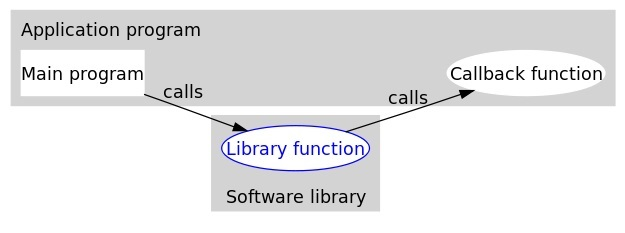
\includegraphics[scale=0.5]{Callback}  

Figura 3: Soluzione frazionaria
\end{center}


Tipicamente le callBack eseguono elaborazioni che saranno inoltrate a Cplex il quale le sfrutta durante l' evoluzione dell' algoritmo di Branch and cut: tali elaborazioni possono essere specifiche del problema che si sta risolvendo aumentando così le performance del programma. Nel programma realizzato sono state utilizzate le callback di Cplex per aggiungere al volo tagli specifici per il problema del Commesso Viaggiatore durante l' evoluzione del Branch and Cut.
Tra le varie CallBack che Cplex mette a disposizione c' è ne sono due particolarmente importanti che saranno oggetto dei successivi paragrafi: la \textbf{LazyCallback} e la \textbf{UserConstraintCallback}.


\vspace{2\baselineskip}
LAZYCALLBACK
\vspace{2\baselineskip}

Durante il processo di risoluzione del Branch-and-cut, ogni volta che Cplex risolvendo il rilassamento continuo in un nodo calcola una soluzione ammissibile il cui costo è inferiore rispetto all' incumbet attuale viene invocata la lazycontraint callback prima di aggiornare l'incumbent, qualora la soluzione intera ha un costo superiore all' incumbent, per il \textit{criterio di bounding} il nodo viene eliminato. Poichè , come più volte ricordato, al modello di partenza non sono stati aggiunti i vincoli di subtour è possibile che la soluzione calcolata da Cplex sia ammissibile per il modello corrente ma contenga dei subtour al suo interno.  Il codice che presenteremo nei prossimi paragrafi sfrutta la lazycontraint callback per consentire a Cplex di aggiornare l' incumbent  solo se la soluzione di un nodo per il quale viene invocata la lazycontraint callback non ha subtour al suo interno, altrimenti all' interno della callback si genera un taglio per ogni sottociclo.

In generale i tagli possono essere \textbf{locali} o \textbf{globali}: mentre i primi hanno validità esclusiva al sottoalbero avente come radice il nodo per la quale sono stati generati , i secondi hanno validità per tutti i nodi dell' albero decisionale e vengono memorizzati in una struttura globale detta \textbf{pool di tagli}. Una volta che un taglio viene aggiunto al pool, se questo può essere rimosso in un secondo momento, poiché ritenuto inefficace, si dice che tale taglio è \textbf{purgeable}. Durante il proseguo della tesi i tagli saranno da considerarsi sempre globali e non purgeable: per tale ragione un taglio con queste caratteristiche è come se fosse aggiunto al modello non potendo essere più violato.
Si osserva che a differenza del metodo Loop una volta che Cplex produce la soluzione ottima questa certamente è ammissibile e corrisponde quindi al tour ottimo che si vuole cercare. A livello implementativo sarà  mostrato sia come installare questa callBack in C\# sia in C poichè questo ci tornerà  utile nel proseguito della tesi.

\vspace{2\baselineskip}
MULTI-THREAD
\vspace{2\baselineskip}

Il software Cplex prima di risolvere il modello interroga il sistema operativo al fine di stabilire il numero di core presenti nel processore e pone il numero di thread al numero di core in esso presenti. Al giorno d' oggi i moderni processori dispongono almeno di due core: risulta quindi utile associare ad ognuno di essi un thread con il compito di risolvere il rilassamento continuo di un nodo dell' albero decisionale. Così facendo si sfrutta al massimo la potenza del processore incrementando in questo modo le performance del programma.  
Nel momento in cui si installa una delle due callback, si ha la possibilità che due thread distinti invochino contemporaneamente la funzione da noi realizzata per aggiungere tagli al modello: qualora tale funzione modifichi variabili che sono condivise fra i vari thread si potrebbe andrebbe incontro ad eccezioni o anomalie  tali da non garantire più la correttezza della soluzione prodotta da Cplex. 
Per evitare queste problematiche, i progettisti di Cplex hanno preferito  settare il numero di thread al valore 1 dopo l' installazione della Lazy o della UserCut callback. Naturalmente tale scelta inficia le performance: si è quindi deciso di riportare il numero di thread al numero di core presenti nel processore prestando attenzione a realizzare un codice thread-safety. Maggiori dettagli di quanto detto sono riportati nei successivi paragrafi.


\vspace{2\baselineskip}
INSTALLAZIONE LAZYCONSTRAINT CALLBACK C\#
\vspace{2\baselineskip}


Per poter installare la LazyConstraintCallback in C\# è prima necessario creare un classe che estenda Cplex.LazyConstraintCallback: tale classe è stata chiamata TSPLazyConsCallback. All' interno di essa è obbligatorio sovrascrivere il metodo Main della classe ereditata: al suo interno sarà realizzato il codice che, a partire dalla soluzione intera calcolata da Cplex in un nodo dell' albero decisionale avente un costo inferiore rispetto all' incumbent attuale, aggiunge per ogni subtour (se presente) il relativo taglio.
Per installare la callback è necessario utilizzare il metodo \textbf{Use} sull' istanza della classe Cplex nella quale è stato definito il modello e passargli come parametro una istanza della classe \textbf{TSPLazyConsCallback}. 
\begin{lstlisting}

cplex.Use(new TSPLazyConsCallback(cplex, instance, process, z, true));

\end{lstlisting}


\textit{[Qui penso possa dare fastidio al prof aver messo direttamente true..conviene secondo me fare una variabile a parte , chiamarla BlockPrint e metterla a true… ]}

I parametri che si vogliono rendere visibili all' interno della classe bisogna passarli come parametro all' atto della creazione dell' istanza della classe TSPLazyConsCallback. L' unico parametro il cui significato non è noto è BlockPrint: essa è una variabile booleano che indica se il grafo di supporto della soluzione intera in corrispondenza della quale è stata invocata la Lazy debba essere o meno stampato a video. Tale parametro è utile poiché la lazy verrà utilizzata anche all' interno di altri  algoritmi per i quali non risulta particolarmente interessante graficare a video il grafo di supporto della soluzione. 
Come accennato nel paragrafo precedente, l' installazione della Lazy setta il numero di thread a 1: per riportare il numero di thread al numero di core è necessario utilizzare i metodi \textbf{SetParam} e \textbf{GetNumCores} entrambi sull' istanza cplex.


\begin{lstlisting}

cplex.SetParam(Cplex.Param.Threads, cplex.GetNumCores());

\end{lstlisting}

Si osserva che, utilizzando la funzione GetNumCores, si è reso il codice indipendente dal numero di core del computer sul quale si andrà poi ad eseguire effettivamente il codice.
Per mostrare a video il grafo di supporto di una soluzione con gnuplot è necessario, come discusso nel paragrafo X,  creare un file avente una determinata struttura. Poiché si è deciso di lavorare in un ambiente multi-thread, potrebbe essere fonte di anomalie creare un unico file accessibile da tutti i thread all' interno del quale quest' ultimi scrivono le coordinate della relativa soluzione intera calcolata.  Qualora almeno due thread nel medesimo istante invocano la callback si ritroverebbero a scrivere sullo stesso file coordinate appartenente a soluzioni differenti. 
Per tale ragione si è realizzato un codice in cui ogni thread che invoca la lazycallback crea un proprio file sul quale scrivere le coordinate della soluzione calcolata. Per far ciò ad ogni file è stato attribuito un nume univoco avente la seguente struttura:


\begin{lstlisting}

instance.InputFile + "_" + nodeId + ".dat"

\end{lstlisting}


dove \textbf{nodeId} risulta essere una stringa che dipende dal nodo sul quale un thread ha invocato la lazy: in particolare rappresenta l' indice del nodo. Per ottenere tale stringa è stato necessario invocare il metodo \textbf{GetNodeId} ereditato dalla classe Cplex.LazyConstraintCallback:


\begin{lstlisting}

string nodeId = GetNodeId().ToString();

\end{lstlisting}

Prima di verificare se la soluzione al suo interno contiene o meno cicli bisogna naturalmente accedere a tale soluzione: a tal fine si deve utilizzare il metodo \textbf{GetValues} ereditato dalla classe Cplex.LazyConstraintCallback il quale riceve in input il vettore z e restituisce per ogni variabile il corrispondente valore.


\begin{lstlisting}

public class TSPLazyConsCallback : Cplex.LazyConstraintCallback
{
	…

	public override void Main()
	{
         double[] actualZ = GetValues(z);
    		…
	}
}


\end{lstlisting}

\textit{[Ho riportato sia il Main che la classe perchè dopo tante parole mi sembrava piu chiaro vedere poi il codice effettivo…]}


Una volta ottenuta la soluzione per verificare se sono presenti cicli e definire i corrispondenti vincoli di subtour si sono utilizzati i metodi \textbf{InitCC} e \textbf{UpdateCC} e le medesime strutture dati ampliamene descritte nei paragrafi X.Y; solo per completezza si riporta il codice realizzato.



 \textit{[Qui non ho capito perchè hai fatto un altro metodo BuildCC che fa le stesse cose di UpdateCC]}


\begin{lstlisting}

List<ILinearNumExpr> ccExprLC = new List<ILinearNumExpr>();
List<int> bufferCoeffCCLC = new List<int>(); ;

int[] compConnLC = new int[instance.NNodes];

Utility.InitCC(compConnLC);

for (int i = 0; i < instance.NNodes; i++)
            {
                for (int j = i + 1; j < instance.NNodes; j++)
                {
                    //Retriving the correct index position for the current link inside z
                    int position = Utility.zPos(i, j, instance.NNodes);

                    //Only links in the optimal solution (coefficient = 1) are printed in the GNUPlot file
                    if (actualZ[position] >= 0.5)
                    {
                        //Updating the model with the current subtours elimination
                        BuildCC(i, j, ccExprLC, bufferCoeffCCLC, compConnLC);

                        if (BlockPrint)
                        {
                            fileLC.WriteLine(instance.Coord[i].X + " " + instance.Coord[i].Y + " " + (i + 1));
                            fileLC.WriteLine(instance.Coord[j].X + " " + instance.Coord[j].Y + " " + (j + 1) + "\n");
                        }
                    }
                }
            }


\end{lstlisting}



Una volta memorizzato l’ i-esimo taglio all’ interno di ccExprLC[i] e bufferCoeffCCLC[i], per aggiungerlo al modello è necessario utilizzare il metodo Add ereditato dalla classe Cplex.LazyConstraintCallback, tale metodo ha come firma:

\begin{lstlisting}

IloRange Add(IloRange cut, int cutmanagement) 

\end{lstlisting}


dove:

\begin{itemize}
	\item \textbf{cut}: Rapprerenta il vincolo che deve essere aggiunto come taglio globale. Il vincolo deve essere lineare.
	\item \textbf{cutmanagement}: Valore intero che indica come il taglio deve essere gestito da Cpex. I possibili valori che può assumere tale parametro solo:
	
	\begin{itemize}
	\item \textbf{0}: Il taglio è aggiunto al rilassamento in maniera permanente.
	\item \textbf{1}: Il taglio è aggiunto al rilassamento, ma può essere eliminato successivamente se Cplex determina che risulta essere inefficiente. Il questo caso di 											parla di taglio \textbf{purgeable}. 
	\item \textbf{2}: Il taglio viene trattato come i tagli generati da Cplex, ossia viene analizzato prima di aggiungerlo al rilassamento.  Qualora, per esempio, Cplex ritiene che esiste 							già un taglio più efficace questo non viene aggiunto.	
	\end{itemize}

\end{itemize}

\textit{[Nella documentazione parlano di rilassamento, secondo me è più giusto pool di tagli]}

Come riportato dalla documentazione, IloRange risulta essere una interfaccia utilizzata per modellare oggetti che rappresentano ranged constraints nel formato:


$$lb <= expr <= ub$$ 


Un oggetto di tipo IloRange può essere ottenuto utilizzando il metodo \textbf{Le} il quale crea e ritorna un vincolo che forza una data espressione ad essere minore o uguale di uno specifico valore. 

\begin{lstlisting}

public IloRange Le(IloNumExpr e, double v)

\end{lstlisting}

dove :

\begin{itemize}
	\item \textbf{e}: Espressione contenente una combinazione lineare delle variabili relative al vincolo..
	\item \textbf{v}: Termine noto del vincolo. 
\end{itemize}


Riportiamo il codice realizzato per aggiungere il taglio:


\begin{lstlisting}

IRange[] cuts = new IRange[ccExprLC.Count];

            if (cuts.Length > 1)
            {
                for (int i = 0; i < cuts.Length; i++)
                {
                    cuts[i] = cplex.Le(ccExprLC[i], bufferCoeffCCLC[i] - 1);
                    Add(cuts[i], 1);
                }
            }

\end{lstlisting}


\textit{[Il codice qui lo modificherei perché memorizziamo nel vettore cuts tutti i tagli ma questo poi non li usiamo mai..aggiungerei direttamente il taglio con Add al modello senza prima memorizzarlo nel vettore]}


\vspace{2\baselineskip}
LAZYCONSTRAINTCALLBACK IN C
\vspace{2\baselineskip}



Per installare la LazyConstraint callback in C è necessario, prima di risolvere il modello, invocare la routine \textbf{CPXsetlazyconstraintcallbackfunc} la cui firma è:

\begin{lstlisting}

CPXsetlazyconstraintcallbackfunc(CPXENVptr env,int(*)(CALLBACK_CUT_ARGS) lazyconcallback, void * cbhandle)

\end{lstlisting}



dove:

\begin{itemize}
	\item \textbf{env}: Espressione contenente una combinazione lineare delle variabili del vincolo.
	\item \textbf{lazyconcallback}: Rappresenta il nome, attribuito dal programmatore esterno, della funzione che viene invocata da Cplex qualora la soluzione del rilassamento continuo di un 										nodo è intera e inferiore dell' incumbent. Come nome è stato scelto myLazyCallBack.
	\item \textbf{cbhandle}: Puntatore ad una struttura dati passata dall' utente contenente dati che devono essere visibili all' interno della callback da noi scritta. Come parametro si è 								 passato il puntatore all' istanza. 
\end{itemize}


Per impostare il numero di thread al numero di core bisogna prima ricavare quanti core il processore dispone; a tal fine si sono utilizzati i metodi \textbf{CPXsetintparam} e \textbf{CPXgetnumcores}.

\begin{lstlisting}

CPXgetnumcores(env, int * nCore);
CPXsetintparam(env, CPXPARAM_Threads, nCore);


\end{lstlisting}


Passiamo ora a descrivere la funzione myLazyCallBack che identifica i subtourElimination e aggiunge i relativi vincoli al modello. Essa, come previsto dal manuale, deve avere la seguente firma:


\begin{lstlisting}

static int CPXPUBLIC myLazyCallBack(CPXCENVptr env, void *cbdata, int wherefrom, void *cbhandle, int *useraction_p)

\end{lstlisting}


La lista dei parametri è definita dai progettisti di Cplex poiché la chiamata alla funzione myLazyCallBack avviene all’ interno del codice di Cplex (non accessibile) da essi realizzato: il programmatore esterno è dunque vincolato nella firma. Passiamo ora a descrivere i parametri di myLazyCallBack:



\begin{itemize}
	\item \textbf{env}: rappresenta l’ istanza dell’ enviroment  con il quale stiamo lavorando.
	\item \textbf{cbdata}: rappresenta il puntatore che è stato passato dall’ utente come parametro all’ atto della installazione della lazy e, come detto, punta all’ area di memoria contenente i dati che verranno utilizzati all’ interno della call back. In c i puntatori hanno un tipo poiché essi puntano sempre al primo elemento contenuto in una area di memoria e grazie al tipo è possibile interpretare correttamente i dati in essa contenuti. I progettisti di Cplex a priori non possono sconoscere il tipo della struttura dati che contiene i parametri utilizzati dall’ utente all’ interno della funzione: per tale ragione questo puntatore è di tipo void.
	\item \textbf{wherefrom}:Definisce da che punto del Branch and bound è stata invocata la funzione, ai fini pratici tale parametro, per la lazy callback è risultato irrilevante. 
	\item \textbf{cbhandle}: puntatore a dati privati utilizzato da Cplex
	\item \textbf{useraction_p}:Puntatore ad un intero che contiene la specifica azione da prendere all’ interno della callback scritta dall’ utente. Tale parametro può assumere i seguenti tre valori:
	
	\begin{itemize}
	\item \textbf{0}: Avente come costante simbolica CPX_CALLBACK_DEFAULT comunica a Cplex che fino a quel punto la callback non ha aggiunto tagli al modello.
	\item \textbf{1}: Avente come costante simbolica CPX_CALLBACK_FAI impone a Cplex di uscire dall' ottimizzazione.
	\item \textbf{2}: Avente come costante simbolica CPX_CALLBACK_SET_comunica a Cplex che sono stati aggiunti tagli.
	\end{itemize}

\end{itemize}


La prima operazione da compiere all' interno della Lazy consiste nell' effettuare un cast al puntatore cbhandle il qui tipo è noto solo al programmatore che ha installato la callback: nel nostro caso il puntatore è di tipo instance per cui si è effettuato il seguente cast:


\begin{lstlisting}

instance *inst = (instance*)cbhandle;

\end{lstlisting}


Successivamente è necessario assegnare al parametro *useraction_p il valore CPX_CALLBACK_DEFAULT.


Per ottenere  la soluzione del rilassamento continuo  è necessario utilizzare il metodo CPXgetcallbacknodex avente come intestazione:

\begin{lstlisting}

int CPXgetcallbacknodex(CPXCENVptr env, void * cbdata, int wherefrom, double * x, int begin, int end) 

\end{lstlisting}


\begin{itemize}
	\item Per quanto riguarda env, cbdata, wherefrom vale la descrizione vista per il metodo myLazyCallBack
	\item \textbf{x}: Array che al termine del metodo conterrà la soluzione intera del rilassamento continuo.
	\item \textbf{begin}: Indica l’ indice della prima variabile di cui si vuole conoscere il valore.
	\item \textbf{end}: Indica l’ indice dell’ ultima variabile di cui si vuole conoscere il valore; poiché vogliamo conoscere il valore di tutte le variabili a begin sarà passato il valore 0 mentre ad end [n*(n-1)/2] – 1.
\end{itemize}

All' atto dell' invocazione del metodo CPXgetcallbacknodex non viene passato come parametro l' array \textbf{bestLb} contenuto in inst ma viene creato un opportuno array chiamato \textbf{xstar}:


\begin{lstlisting}

double *xstar = (double*)malloc(inst->nCols * sizeof(double));

\end{lstlisting}

Risulta necessario far ciò al fine di realizzare un codice che sia thread-safety: poiché inst è un puntatore accessibile a tutti i thread esiste il rischio che più thread contemporaneamente sovrascrivano il contenuto di bestLb ottenendo un bestLb che contiene coordinate appartenenti a soluzioni differenti.
Ricavata la soluzione è necessario verificare se essa ha al suo interno dei sottocicli e in tal caso procedere con l’ aggiunta dei un vincoli di subtour per ogni subtour. A differenza di quanto fatto in C\#, per determinare i subtour, si è utilizzato Concorde\footnote{ In particolare la funzione CCcut_connect_components } che verrà presentato nel paragrafo successivo: poiché il codice che sfrutta Concorde per il calcolo dei vincoli di subtour si ritrova anche per la user cut callback la sua presentazione è rimandata al paragrafo X.Y.
Una volta che abbiamo aggiunto tagli, è necessario impostare il parametro *useraction_p al valore CPX_CALLBACK_SET, al fine di comunicare a Cplex che sono stati aggiunti tagli. 


\vspace{2\baselineskip}
MULTI-THREAD
\vspace{2\baselineskip}

La Usercut callback viene invocata da Cplex ogni volta che la soluzione del rilassamento continuo in un nodo dell' albero decisionale risulta frazionaria; qualora risulti intera viene invocata la Lazy discussa nel paragrafo precedente.  Aggiungere tagli  in un nodo è utile poiché migliora il lower bound rendendo il branch-and-cut più efficace, tuttavia un accumulo eccessivo di tagli peggiora le performance: di questo thread-off si è tenuto conto durante la realizzazione del codice.  
Ciò che dovremmo andare ad implementare è un separatore che, ricevendo in ingresso la soluzione x* con almeno una componente frazionaria, fornisca in uscita un insieme S \subsetneq{V}, |S| \geq 2 tale per cui:

f1


Tale sottoinsieme non è facilmente individuabile come nel caso di soluzione intere in cui era sufficiente individuare le componenti connesse. Per esempio in Figura 3 si è riportato il supporto di una soluzione x* frazionaria ove i lati colorati di rosso, blu e grigio indica che la corrispondente variabile ha come valore 1, 0.5 , 1. 5.

\begin{center}
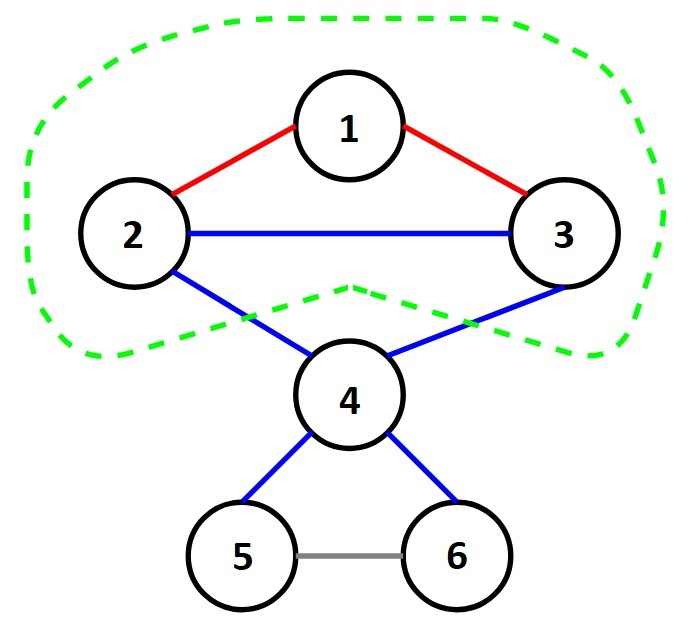
\includegraphics[scale=0.5]{SoluzioneFrazionaria}  

Figura 3: Soluzione frazionaria
\end{center}

Tale grafo risulta connesso; tuttavia è presente un sottoinsieme S = {1,2,3} per cui vale f1.

Una seconda formulazione equivalente di f1 risulta essere la seguente:

f2

Si osserva che il primo membro della disuguaglianza può essere visto come la capacità di una sezione di una rete di flusso se si interpretano le x* come le capacità della rete.
E' possibile calcolare una sezione di capacità minima risolvendo un problema di max flow che sappiamo essere un problema di programmazione lineare e quindi risolubile utilizzando un algoritmo polinomiale.
Poichè però la sezione di capacità minima dipende dal nodo sorgente s e dal nodo di destinazione t, si devono in realtà risolvere n-1 problemi di max flow: per tale ragione è stato preferito utilizzare il software ottimizzato Concorde per identificare la sezione di capacità minima quando la soluzione del rilassamento continuo è frazionaria. 

\vspace{2\baselineskip}
CONCORDE
\vspace{2\baselineskip}

Concorde è un software, sviluppano in linguaggio c da David Applegate, Robert E. Bixby, Vašek Chvátal, e William J. Cook, specializzato nella risoluzione ottimizzata di istanze del problema del commesso viaggiatore. Concorde risulta un software open source solo se utilizzato a fini accademici e i sorgenti, contenuti in un file zip, sono scaricabili utilizzando il seguente link:




Per poter utilizzare Concorde è stato prima necessario installarlo. In ambiente Windows è necessario importare ogni singolo file .c e .h che appartiene alla distribuzione: al fine di importare il minor numero possibile di file sono stati selezionati e importati solo i file che consentono di utilizzare le funzioni di cui si necessita. I file che si sono inclusi nel progetto sono:


\begin{itemize}
	\item \textbf{allocrus.c}
	\item \textbf{connect.c}
	\item \textbf{cut_st.c}
	\item \textbf{mincut.c}
	\item \textbf{shrink.c}
	\item \textbf{sortrus.c}
	\item \textbf{urandom.c}
	\item \textbf{cut.h}
	\item \textbf{machdefs.h}
	\item \textbf{macrorus.h}
	\item \textbf{util.h}
	\item \textbf{end}
\end{itemize}

Affinché il programma compili, è necessario effettuare le seguenti modifiche:

\begin{itemize}
	\item \textbf{allocrus.c}: All' interno dei file allocrus.c e util.h è necessario importare tramite il comando import il file malloc.h.
	\item \textbf{connect.c}: All' interno del file machdefs.h è necessario eliminare l' inclusione al file config.h.
\end{itemize}

\textit{[….Parlerei direttamente qui della DLL….]}


\vspace{2\baselineskip}
INSTALLAZIONE USERCUT CALLBACK
\vspace{2\baselineskip}


Per installare la usercut callback è necessario utilizzare la routine CPXsetusercutcallbackfunc la cui firma è:


\begin{lstlisting}

int CPXsetusercutcallbackfunc (CPXENVptr env, int(*)(CALLBACK_CUT_ARGS) lazyconcallback, void * cbhandle)

\end{lstlisting}



I parametri sono i medesimi descritti per la funzione CPXsetlazyconstraintcallbackfunc che è necessario comunque installare al fine di garantire la correttezza. Infine è sempre necessario reimpostare in numero di thread al numero di core presenti nel processore utilizzando le note funzioni \textbf{CPXgetnumcores} e \textbf{CPXsetintparam}:


\begin{lstlisting}

CPXgetnumcores(env, &nCore);
	
CPXsetintparam(env, CPXPARAM_Threads, nCore);

\end{lstlisting}



\vspace{2\baselineskip}
FUNZIONE myUserCutCallBack
\vspace{2\baselineskip}

La funzione che viene invocata da Cplex in corrispondenza di una soluzione frazionaria è stata chiamata myUserCutCallBack: la sua firma, analogamente a quanto visto per la LazyCallBack, ci viene imposta dai progettisti di Cplex.

\begin{lstlisting}

int CPXPUBLIC myUserCutCallBack(CPXCENVptr env, void *cbdata, int wherefrom, void *cbhandle, int *useraction_p)

\end{lstlisting}

II significato dei parametri di ingresso di tale funzione è noto poiché tutti i parametri sono già stati descritti nel paragrafo X.Y. [ sono i medesimi descritti per la myLazyCallBack.]


Esattamente quanto visto per la lazy callback, anche qui all' inizio è necessario settare il parametro *useraction_p al valore CPX_CALLBACK_DEFAULT. 


Cplex, una volta calcolata una soluzione frazionara genera in automatico dei propri tagli (per esempio di Gomory). Quando il parametro wherefrom risulta pari a CPX_CALLBACK_MIP_CUT_LAST significa che Cplex non genererebbe più tagli e all’ iterazione successiva procederebbe ad effettuare l’operazione di branching: solo in questa condizione risulta conveniente generare vincoli caratteristici del problema che si sta risolvendo. Qualora il parametro wherefrom risulti diverso da CPX_CALLBACK_MIP_CUT_LAST, il metodo effettua un return 0 senza eseguire alcuna operazione, altrimenti come già discusso per la lazy, è necessario recuperare il puntate all’ istanza.
A livello pratico, come intuitivamente è facile capire, aggiungere ad ogni nodo dell’ albero decisionale dei tagli(i quali si sommano ai tagli che Cplex genera in automatico) risulta una scelta sconsigliata che riduce in maniera drastica le performance di Cplex. Per tale ragione si è deciso di realizzare un codice che aggiunge i vincoli di subtour in un nodo nel quele viene invocata la UserCutCallback con una probabilità p = 0,1. Per realizzare ciò si è ricavato, utilizzando la funzione CPXgetcallbacknodeinfo, l’ indice del nodo sul quale tale funzione è stata invocata e solamente quando il resto della divisione per 10 di tale indice risulta nullo si aggiungono i vincoli al nodo. Successivamente invocando la nota funzione CPXgetcallbacknodex si ottiene la soluzione frazionaria. Prima di procedere con l’ analisi del cuore del metodo, riportiamo il codice fin qui discusso:


\begin{lstlisting}

*useraction_p = CPX_CALLBACK_DEFAULT;
	
int nodecount = 0;
CPXgetcallbacknodeinfo(env, cbdata, wherefrom, 0, CPX_CALLBACK_INFO_NODE_DEPTH, &nodecount);
	
if (wherefrom == CPX_CALLBACK_MIP_CUT_LAST 
{
	instance *inst = (instance*)cbhandle;
		
	double *xstar = (double*)malloc(inst->nCols * sizeof(double));

 	if ((nodecount % 10) != 0))//------------------------------------------------------------------------CORRETA RISPETTO A QUELLA PRESENTE NEL PROGRAMMA
		return 0;

	if (CPXgetcallbacknodex(env, cbdata, wherefrom, xstar, 0, inst->nCols - 1))
	{
		free(comps);
		free(compscount);
		free(xstar);
		free(elist);
		return 1; 
		}
	…
}

\end{lstlisting}


Per aggiungere eventuali vincoli di subtour è necessario invocare in un primo momento la funzione CCcut_connect_components la quale identificare le componenti connesse di una soluzione, essa sia intera o frazionaria. Con il termine identificare si intende che determina per ogni componente quanti e quali nodi da essa costituita.

Illustriamo i parametri che tale funzione riceve in input, si osserva che mentre i primi 4 parametri costituiscono l' effettivo input della funzione i rimanenti 3 sono i parametri che esse setta e quindi possono essere visti come l' output della funzione:

\begin{itemize}
	\item \textbf{ncount}:rappresenta il numero di nodi del grafo;
	\item \textbf{econut}:rappresenta il numero di lati del grafo, ossia ncount*(ncount-1)/2
	\item \textbf{*elist}:vettore avente dimensione 2 * econut. Tale vettore contiene al suo interno tutti i lati del grafo caratterizzati dai nodi sul quale esso incide memorizzati in locazioni consecutive dell’ array. Vedremo in seguito il codice realizzato per popolare questa struttura dati.
	\item \textbf{*x}:soluzione per la quale si desiderano individuare le componenti connesse
	\item \textbf{*ncomp}:rappresenta il numero di componenti connesse.
	\item \textbf{**compscount}:vettore di vettori contenenti il numero di nodi per ciascuna componente connessa, in modo che compscount[i] contenga il numero di nodi presente nell’ i-esima componente connessa
	\item \textbf{**comps}:vettore di vettori contenenti gli indici dei nodi presenti all' interno delle componenti.
\end{itemize}


Il codice realizzato per popolare elist risulta essere il seguente:


\begin{lstlisting}

int loader = 0;
for (int i = 0; i < inst->nNodes;  i++)
{
	for (int j = i + 1; j < inst->nNodes;  j++) 
	{
	    elist[loader++] = i;
	    elist[loader++] = j;
	}
}

\end{lstlisting}

Nonostante non fosse necessario, per rendere il codice maggiormente leggibile si è deciso definire variabili e puntatori con il medesimo nome con i quali sono poi utilizzati all’ interno di CCcut_connect_components.

\begin{lstlisting}

int *compscount = (int*)malloc(inst->nMaxCuts * sizeof(int));		
int *comps = (int*)malloc(inst->nNodes * sizeof(int)); 
int nLati = ((inst->nNodes - 1)*inst->nNodes / 2);
int *elist = (int*)malloc((nLati * 2) * sizeof(int));		
int ncomp; 

\end{lstlisting}


\begin{lstlisting}
if (CCcut_connect_components(inst->nNodes, nLati, elist, xstar, &ncomp, &compscount, &comps))
printError(" error in CCcut_connect_components() inside fractcutusercallback");
\end{lstlisting}
 
Utilizzando i vettori ncomp compscount, comps è stato possibile realizzare un codice in grado di definire i vincoli di subtour per ogni componente connessa e successivamente di inserirli nel pool dei tagli tramite la funzione \textbf{CPXcutcallbackadd} la cui firma è:

\begin{lstlisting}

CPXcutcallbackadd(CPXCENVptr env,void * cbdata,int  wherefrom,int  nzcnt, double  rhs,int sense,int cutind,double const *  cutval, int purgeable);

\end{lstlisting}


\begin{itemize}
	\item \textbf{env,cbdata,wherefrom}: Questi sono parametri noti già discussi nella callback myLazyCallback
	\item \textbf{nzcnt}:Numero di coefficienti diversi da zero del vincolo
	\item \textbf{rhs}:Definisce il termine noto del vincolo
	\item \textbf{sense}:Può assumere i seguenti valori:


	\item \textbf{cutind}:Array di  nzcnt elementi contenenti gli indici delle variabili presenti nel vincolo
	\item \textbf{cutval}:Array di  nzcnt elementi contenenti i corrispondenti valori dei coefficienti
	\item \textbf{purgeable}:Valore intero che specifica come Cplex tratta il taglio,i possibili valore che possono essere passati in input sono:
	
	\begin{itemize}
	\item \textbf{CPX_USECUT_FORCE}:Il taglio una volta aggiunto al rilassamento non può essere più rimosso
	\item \textbf{CPX_USECUT_PURGE}:Il taglio è aggiunto al rilassamento ma può essere eliminato in un secondo momento se giudicato inefficiente
	\item \textbf{CPX_USECUT_FILTER}: Il taglio viene trattato come un taglio generato da Cplex il quale prima di aggiungerlo al rilassamento lo analizza e può decidere di non inserirlo 
	nel rilassamento(per esempio è già presente un taglio più efficiente)
	
	\end{itemize}

    
\end{itemize}

Per aggiungere un taglio per ogni componente connessa è stato necessario popolare i vettori cutval, cutind e la variabile nzcnt opportunamente sfruttando le informazioni contenute in compscount, comps. Per stabilire quali nodi appartengono alla t-esima componente connessa si sono dichiarate due variabili intere k1,k2 che contengono sistematicamente l' indice del primo e dell' ultimo nodo dei nodi appartenenti alla t-esima componente connessa memorizzati in comps. Si osserva che k2 è stato dichiarato pari a -1 poichè gli indici all' interno dell' array parto da 0. 

\begin{lstlisting}

	if (ncomp > 1)
		{
			int k1 = 0;
			int k2 = -1;

			for (int c = 0; c < ncomp; c++)
			{
				int dimIndexValue = compscount[c] * (compscount[c] - 1) / 2; 
				int *cutind = (int*)malloc(dimIndexValue * sizeof(int));
				double *cutval = (double*)malloc(dimIndexValue * sizeof(double));
				int nzcnt = 0;

				
				k2 += compscount[c];

				for (int i = k1; i < k2; i++)
				{
					for (int j = i + 1; j <= k2; j++)
					{
						cutval[nzcnt] = 1.0;
						cutind[nzcnt] = xPos(comps[i], comps[j], inst);
						nzcnt++;
					}
				}

				k1 = k2 + 1;	
				
				CPXcutcallbackadd(env, cbdata, wherefrom, nzcnt, compscount[c] - 1, 'L', cutind, cutval, CPX_USECUT_FORCE);

				*useraction_p = CPX_CALLBACK_SET; 
				free(cutind);
				free(cutval);
			}

			free(elist);
			free(comps);
			free(compscount);
			free(xstar);


			return 0;
		}

\end{lstlisting}


Nel caso in cui la soluzione presenta una sola componente connessa, come in Fig. X, invocando la funzione \textbf{CCcut_violated_cuts} di Concorde è possibile individuare gli insiemi S che soddisfino la disuguaglianza (f2) : una volta individuato S risulta banale inserire il relativo vincolo di subtour. In particolare CCcut_violated_cuts è una funzione in grado di individuare sezioni di capacità inferiori ad una certa soglia. Descriviamo i 7 parametri che tale funzione riceve in input, si osserva che a differenza della funzione CCcut_connect_components i parametri sono effettivamente tutti di input:


\begin{itemize}
	\item \textbf{ncount}: int ecount, int *elist: Il loro significato è già stato descritto per la CCcut_connect_components
	\item \textbf{dlen}: vettore contenente la capacità di ogni lato. 
	\item \textbf{cutoff}:[Questo è il termine noto della disequazione f2, non ho capito perchè devo togliere a 2 un EPSILON, così è scritto nel pdf condiviso dal prof che si chiama 		RO2_TSPutilities]
	\item \textbf{(*(doit_fn)(double,int,int *,void *) }:La peculiarità di questa funzione è rappresentata dal fatto che, quando viene invocata, viene installata una callback, il cui nome è rappresentato dal valore di questo parametro, che sarà evocata da Concorde tutte le volte che quest' ultimo individua un sottoinsieme S che soddisfa f2. Si osserva che i parametri di ingresso della callback, che si è chiamata doitFuncConcorde, sono stabiliti dai programmatori che hanno realizzato Concorde poiché essa viene invocata all' interno del codice da essi realizzato: sfruttando tali parametri all' interno di doitFuncConcorde si inserirà il relativo taglio al nodo. Tale parametri possono considerarsi l' output della funzione.
	\item \textbf{pass_param}:puntatore alla struttura dati, di tipo InputCC, contenente variabili e puntatori che devono essere accessibili all’ interno della callback 
\end{itemize}

Poiché all' interno della callback si desidera aggiungere tagli, per poterlo fare si ha la necessità di accedere alle variabili e puntatori che la funzione CPXcutcallbackadd richiede come parametri di ingresso. Per tale ragione la struttura inputCC contiene al suo interno le seguenti variabili e puntatori tutti ampliamente descritti nei paragrafi precedenti:

\begin{lstlisting}

typedef struct 
{ 
	instance *inst;
	CPXCENVptr env;
	void *cbdata;
	int wherefrom;
	int *useraction_p;
} inputCC;


\end{lstlisting}


Passiamo ad analizzare il codice di doitFuncConcorde, la cui intestazione è:

\begin{lstlisting}

int doitFuncConcorde(double cutValue, int cutcount, int *cut, void *inParam)

\end{lstlisting}

dove:

\begin{itemize}
	\item \textbf{cutValue}: Rappresenta il valore del taglio,
	\item \textbf{cutcount}: Rappresenta il numero dei nodi,
	\item \textbf{cut}: Array contenente l' indice associato ai nodi,
	\item \textbf{inParam}:struttura dati passata in input dal programmatore esterno.
\end{itemize}

Come ormai è noto, è necessario recuperare il puntatore alla struttura dati fornita in input alla callback:

\begin{lstlisting}

inputCC *in = (inputCC*)inParam;

\end{lstlisting}

Per aggiungere il taglio è necessario utilizzare la funzione CPXcutcallbackadd: si sono così definiti due array di interi cutind e cutval contenenti rispettivamente gli indici delle variabili che costituiscono il taglio e il relativo coefficiente. Si è inoltre dichiarata una variabile intera nzcnt che contiene il numero di variabili che partecipano taglio. 

\begin{lstlisting}

int dimIndexValue = inst->nNodes * (inst->nNodes - 1) / 2; 

int *cutind = (int*)malloc(dimIndexValue * sizeof(int));
double *cutval = (double*)malloc(dimIndexValue * sizeof(double));
\end{lstlisting}


Poiché il taglio è composto dalle variabili associate ai lati aventi entrambi gli estremi in S, l’ indice di tutte le variabili è ricavabile utilizzando la funzione xPos la quale riceve in input ad ogni iterazione un lati [i,j] con i<j e i,j nodi contenuti in cut. 

\begin{lstlisting}

int nzcnt = 0;

	for (int i = 0; i < cutcount - 1; i++)
	{
		for (int j = i + 1; j <= cutcount - 1; j++)
		{
			int n1 = cut[i];
			int n2 = cut[j];
			cutind[nzcnt] = xPos(n1, n2, inst);
			cutval[nzcnt] = 1.0;
			nzcnt++;
		}
	}
CPXcutcallbackadd(in->env, in->cbdata, in->wherefrom, nzcnt, cutcount - 1, 'L', cutind, cutval, CPX_USECUT_FORCE);

*in->useraction_p = CPX_CALLBACK_SET;

free(cutind);
free(cutval);

return 0;

\end{lstlisting}

\end{document}